\chapter{Problem Definition: Developmental AI}
\minitoc

The present research expands upon the standard \ai methods presented in the previous chapter, with the aim of investigating fundamental inquiries within the domain of \gls{Developmental Artificial Intelligence}. Developmental \ai is a multidisciplinary field that integrates principles from artificial intelligence, developmental psychology, linguistics, and neuroscience to simulate and analyze the cognitive development of sensorimotor, cognitive, and cultural structures, both at the level of artificial agents and at the level of populations. While standard \ai paradigms are structured around precise and formal problems addressed by algorithmic contributions, developmental \ai strives to create machine systems that can learn in an autonomous, autotelic, and open-ended manner, similar to the way children learn. In this research the specific questions that we investigate are: 1) How do cultural conventions emerge through interactions among agents in social contexts? 2) How can autotelic artificial agents utilize cultural conventions to acquire open-ended skill repertoires? These questions can be approached through the lens of self-organization theory. Specifically, this study will examine: 1) the self-organization of conventions, or language, among agents, and 2) the role of cultural conventions in the self-organization of agents' developmental trajectories. 

The initial part of this section (\sect{sec:self-orga}) outlines the fundamental concept of self-organization, encompassing the development of cultural conventions and the formation of individual trajectories. A typology of the language formation problem is then presented in \sect{sec:self-orga-lang}, which provides us a structured approach to categorizing our two first research investigations (presented in \sect{sec:self-orga-lang-prob-def}), namely the self-organization of graphical sensory-motor language, and the formation of cultural convention in the Architect-Builder problem. These contributions will be developed in Part~\ref{part:formation} of this manuscript. Then, \sect{sec:self-orga-traj} describes the open-ended formation of skill repertoire and introduces the autotelic \rl framework. The autotelic \rl framework will serve as a basis to explore the role of cultural conventions in the self-organization of developmental trajectories. We outline our contributions in \sect{sec:problem-def-vygo} and detail them in Part~\ref{part:exploitation} of this manuscript. 

\section{Self-organization Theory}
\label{sec:self-orga}
Self-organization is a term now used in a variety of sciences that can be described with the following definition:
\begin{tcolorbox}
\small
\paragraph{Definition}
\gls{Self-organization} is a process by which spontaneously ordered patterns and structures emerge from the interactions of the many constituents of a system without the need for central control or external guidance. Crucially, the emergent global structure of self-organizing systems has different properties than its local constituents.
\end{tcolorbox}

Paradoxically, the notion of \textit{emerging order} draws its origin from the study of chaos and was originally used to describe thermodynamical systems that spontaneously organize themself from complex chaotic interactions. The theory of self-organization was formalized by cybernetician \citet{ashby1962self}. Borrowing concepts from dynamical system theory, he stated that any complex dynamical systems organize themselves around specific 'attractors' within a vast landscape of possible states. These attractors are stable equilibrium points and may be multiple for a given system. An intuitive explanation of attractors, proposed by \citet{dilts1995nlp}, is given in \fig{fig:youngoldlady}. It illustrates how our complex perception system can fall into different attractors when presented with an illusion. In one case, we see a young woman wearing a necklace looking up to the left, in the other we perceive an old woman leaning slightly forward. This illustration also demonstrates that certain attractors may be difficult to reach. Indeed, when looking at \fig{fig:youngoldlady} we often rapidly converge to one attractor and have difficulty escaping it to organize our perception around the other. Finding an attractor requires exploring the landscape of possible states. For this, noise and stochasticity can help as described by \citet{vonFoerster2003}:
\begin{quote}
   	``\textit{I think it is favorable to have some noise in the system. If a system is going to freeze into a particular state, it is inadaptable and this final state may be altogether wrong. It will be incapable of adjusting itself to something that is a more appropriate situation.}''
\end{quote}
\begin{figure}[!h]
\centering
\begin{tabular}{cc}
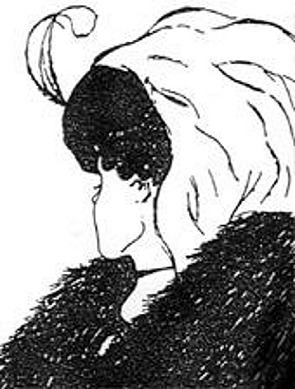
\includegraphics[width=.2\textwidth]{problem_def/Youngoldwoman.jpg}	& 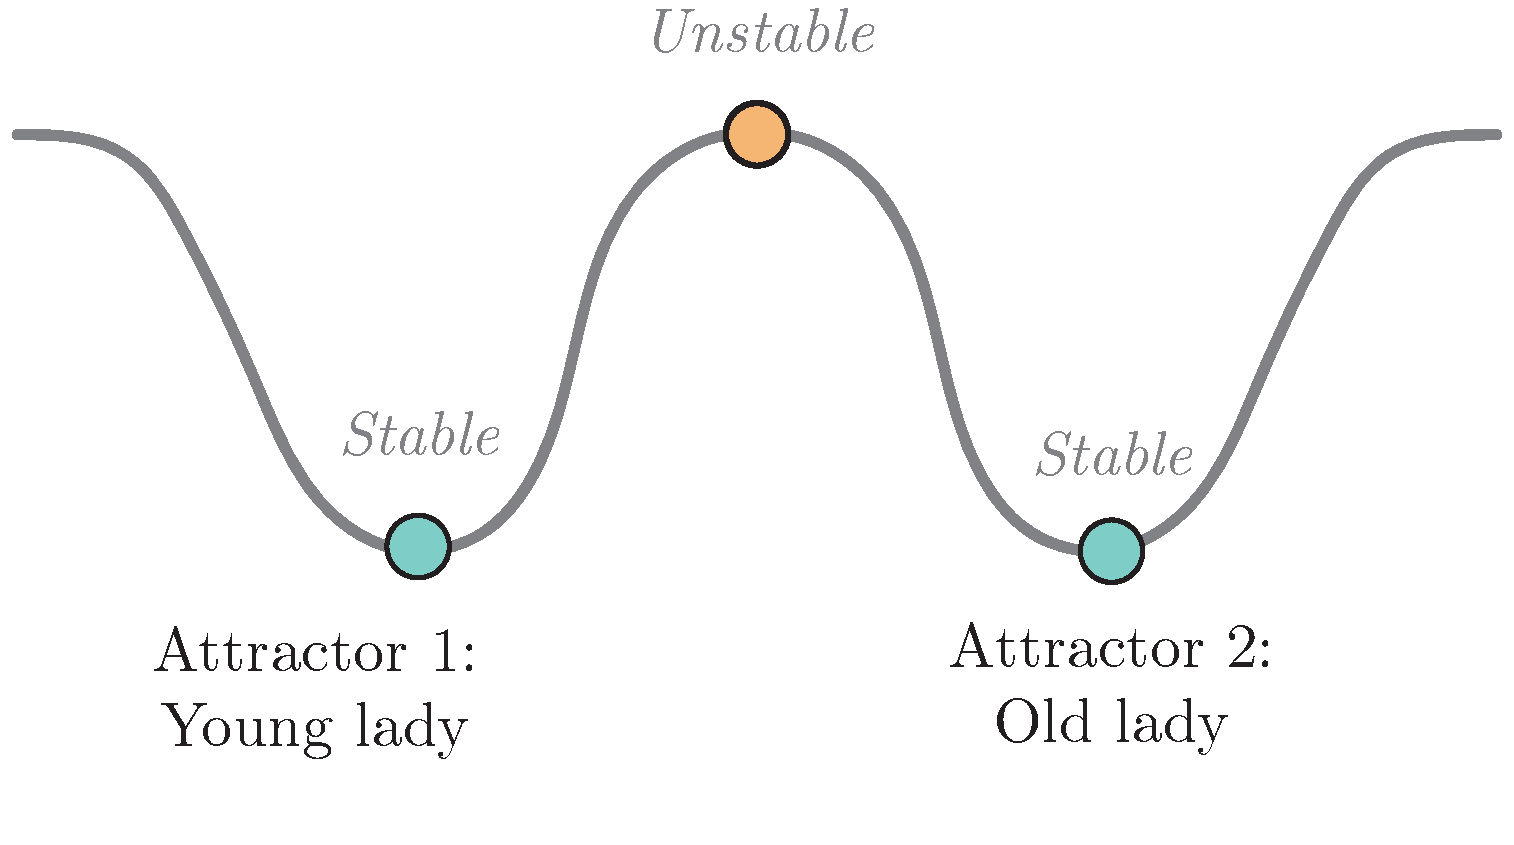
\includegraphics[width=.45\textwidth]{problem_def/stability_plot_yougoldwoman.pdf} \\
(a) & (b)
\end{tabular}
\caption{(a) My Wife and My Mother-In-Law, by the cartoonist W. E. Hill, 1915 (b) Stability plots illustrating the two attractors of the cartoon as proposed by~\citet{dilts1995nlp}}
\label{fig:youngoldlady}
\end{figure}

As displayed in \fig{fig:example_self_org}, nature is full of examples of self-organizing systems. Physical systems exhibit self-organizing behavior through the formation of patterns, such as the longitudinal stripes of sand dunes or the crystalline structure of snowflakes. Similarly, biological systems display self-organizing behaviors\citep{camazine2001self-organization}, as exhibited in the social organization of fish schools and insect swarms, as well as in their ability to collectively adapt to and modify their environment when termites construct mounds and bees build their hives.
%
\begin{figure}[!h]
\small
\centering
\begin{tabular}{c}
	(a) Physical self-organizing systems\\
	
\includegraphics[width=.6\textwidth]{problem_def/self_organizing_physical.pdf}\\
	(b)Biological self-organizing systems\\
	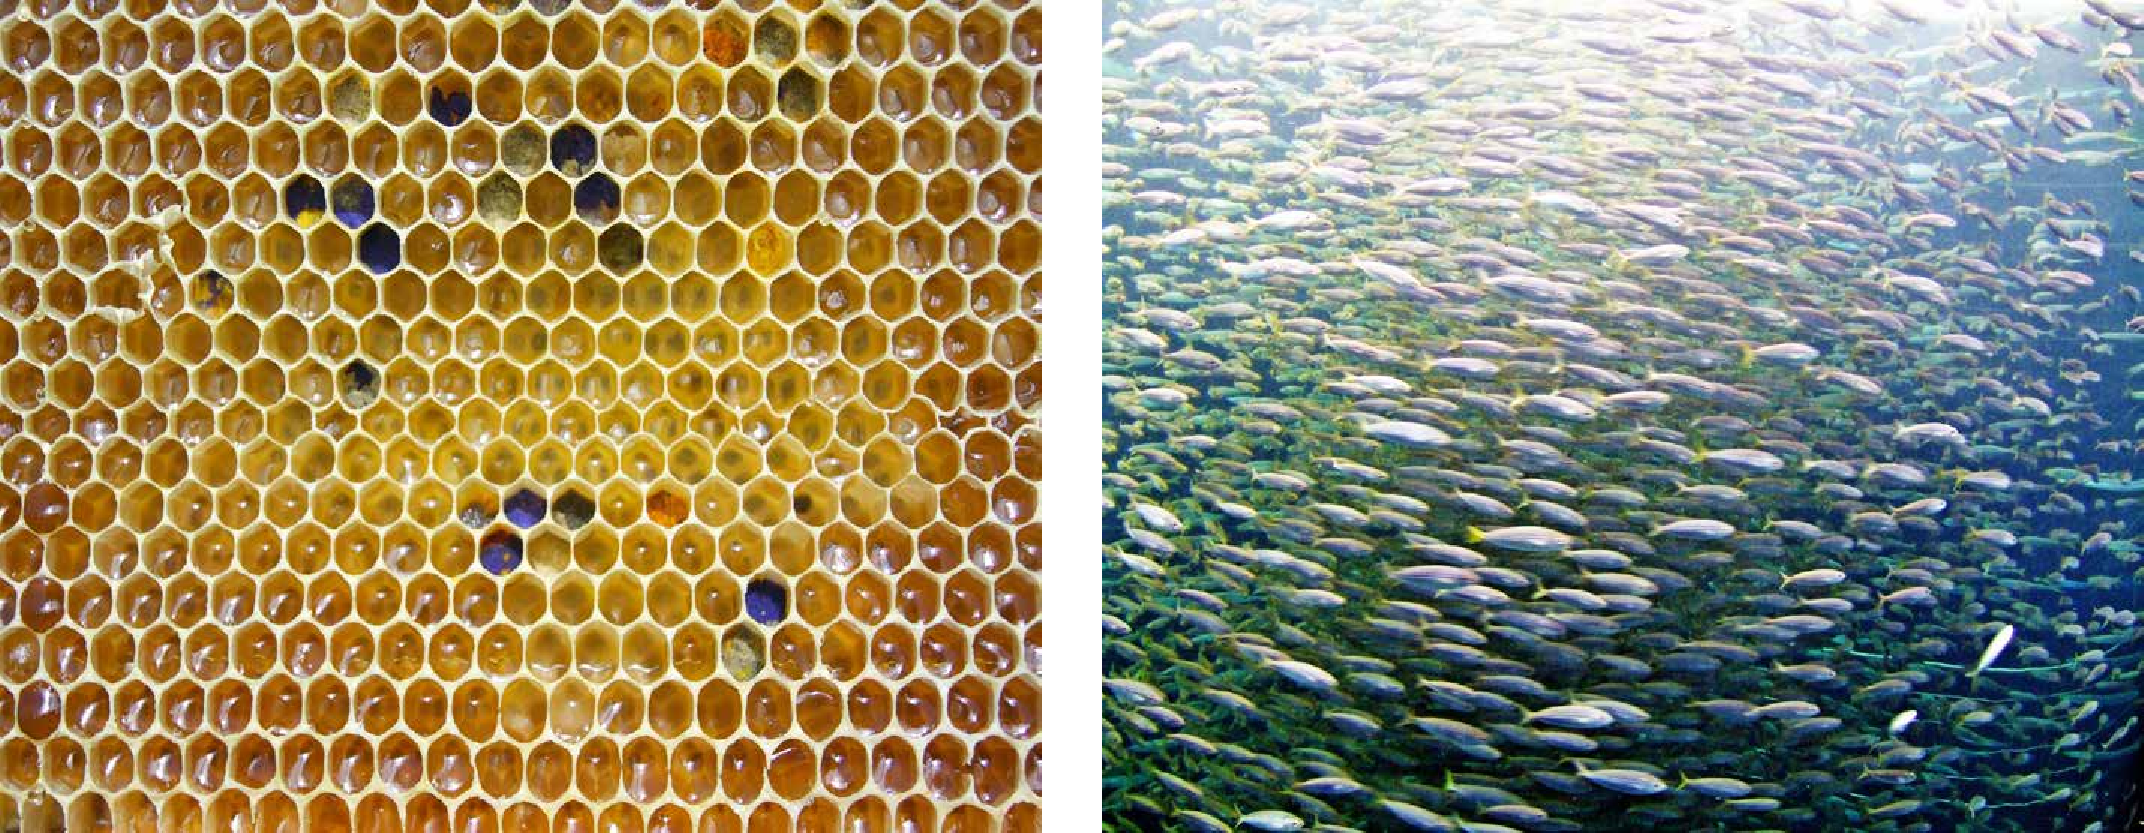
\includegraphics[width=.6\textwidth]{problem_def/self_organizing_biological.pdf}
\end{tabular}
\caption{Example of self-organizing systems (a) sand dunes in Namibia and crystal structure of snow ice; and (b) a bee comp and a fish school. Images are royalty-free and obtained from \url{pixabay.com}}
\label{fig:example_self_org}	
\end{figure}

Self-organization also enables creative technical innovation such as the development of self-organizing traffic lights~\citep{ferreira2010self-organized}: lights that can adapt to changing traffic conditions through local interactions, rather than relying on communication or external signals. Self-organization is particularly well suited for the problem of traffic light regulation because traffic conditions change constantly. Thus, the problem at hand requires adaptation, a property well captured by self-organization theory.

\paragraph{Self-organization in Developmental AI}

Developmental \ai problems can be formulated as adaptive problems where one or more agents and the environment are coupled dynamical systems whose interactions are responsible for the agents' behavior~\citep{beer1995dynamical}. In this research, we propose to use the language of dynamical systems and the theory of self-organization to formalize the two fundamental problems of this research.

 First, the problem of the emergence of cultural convention among artificial agents can be analyzed as the self-organization of a language community~\citep{steels1995selforganizing,oudeyer2005selforganization}. A cultural convention is thus an attractor of a language community: when multiple agents interact, variations of language behaviors are attracted to an equilibrium state because the more members of a community adopt a particular convention, the stronger the convention becomes. We will present several approaches that model Language formation in \sect{sec:self-orga-lang}. 

Second, the problem of autonomous skill acquisition can be framed as the self-organization of agents' trajectories where agents use internal mechanisms to develop rather than being controlled by hierarchical top-down control~\citep{pfeifer2007robotics}. In this context, agents develop and grow repertoires of skills via internal drivers and physical interactions with their environment. These internal drivers, referred to as intrinsic motivations~\citep{oudeyer2005selforganization}, allow agents to self-organize their behavior into developmental trajectories and enable them to acquire increasingly complex skills. We will explore the open-ended formation of skill repertoires and present the autotelic approach as a solution to it in \sect{sec:self-orga-traj}. We will build on autotelic \rl to propose a new vision in developmental \rl where agents also leverage social interactions to augment their autonomous learning capabilities

Our two research investigations are at the intersection between the standard \ai paradigms (presented in the previous chapter) and fundamental questions within the field of developmental \ai. We propose to study them in the next two following questions. Before clearly formalizing our two problems, we survey related implementations at the convergence of standard and developmental \ai, namely the computation language formation framework (\sect{sec:self-orga-lan-context}) and the autotelic \rl problem (\sect{sec:self-orga-traj-context}).

\newpage
\section{Self-organisation of Cultural Convention: the Language Formation Problem}
\label{sec:self-orga-lang}

\subsection{Computational Models of Language Formation}
\label{sec:self-orga-lan-context}
The study of the origin of language has been a subject of interest and debate among various academic disciplines, including linguistics, archaeology, biology, and anthropology. In this section, we will shortly present the predominant theories on Language formation and explore how artificial agents can help experiment with them. For a thorough review of the synthetic modeling of language origins see \citet{steels1997evolution}. There are three predominant theories on the origin of language:
\begin{enumerate}[noitemsep]
\item The \textit{Genetic evolution theory} postulates that language, just like biological complexity,  is the result of natural selection. According to this theory, humans have an innate language organ inside their brains that contains universal rules helping them learn a language during their development. This claim is backed by the famous poverty of stimulus argument which asserts that children do not observe sufficient data to explain their ability to acquire natural language~\citep{chomsky1975reflections}. The genetic evolution theory thus implies that there exist language genes that code for the language organ and that language is preserved due to genetic transmission. 
\item The \textit{Adaptation and self-organization theory} on the other hand supposes that language is preserved in the memories of individuals and transmitted through cultural and social interactions during imitation and acquisition processes. In the adaptation hypothesis, there is no language organ but rather a variety of cognitive and motor primitives that facilitate language formation. 
\item The \textit{Genetic assimilation theory} assumes that language is the result of dual dynamics that both involve cultural and genetic interactions. The genetic assimilation hypothesis is also known as the Baldwin effect. It states that learned behaviors that confer a selective advantage can become genetically encoded over time.  The genetic assimilation theory proposes that initially, humans did not have an innate language structure and that the first forms of language were acquired through adaptation only. But, if the speed of language acquisition played a role in selection, genetic assimilation would have facilitated the development of language acquisition devices.
\end{enumerate}

\paragraph{Language formation with Artificial Agents}

The study of language emergence can benefit greatly from the utilization of agent-based modeling and simulation~\citep{Hurford1989BiologicalEO,birghton2002compositional,cangelosi2002simulating,steels2015talkingheads,kirby2014iterated}. \textit{Computational Experimental Semiotics}~\citep{galantucci2011experimental} is a field that analyzes the numerous factors that contribute to language emergence by examining a population of simulated agents engaging in two distinct types of interaction: \textit{linguistic} and \textit{genetic interactions}. When two agents take part in linguistic interaction, they are in turn speakers and listeners and respectively produce and receive messages describing a context. To study the formation of meanings, linguistic interactions occur within physical environments that contain objects and embodied situations~\citep{steels2012grounded}. Depending on the communicative success of linguistic interactions, agents can update their internal state and adapt to their artificial peers. To investigate the impact of population dynamics, the studied population is open: new agents enter, and others leave. These new agents, generated through genetic interactions and subject to potential mutations, introduce an element of novelty into the system. Finally, in order to obtain realistic models, the population should be studied as a distributed multi-agent system, i.e. there should not be any main global agent that acts over the entire population. Moreover, just like humans cannot enter the brain of others, agents should not be able to access each other's internal states.  A diagram of interactions as well as a high-level algorithmic implementation of the Language formation framework is provided in \fig{fig:language_acquisition_framework} and Alg.~\ref{alg:langage-acquisition}.
\begin{figure}[!h]
\centering
\vspace{-.5cm}
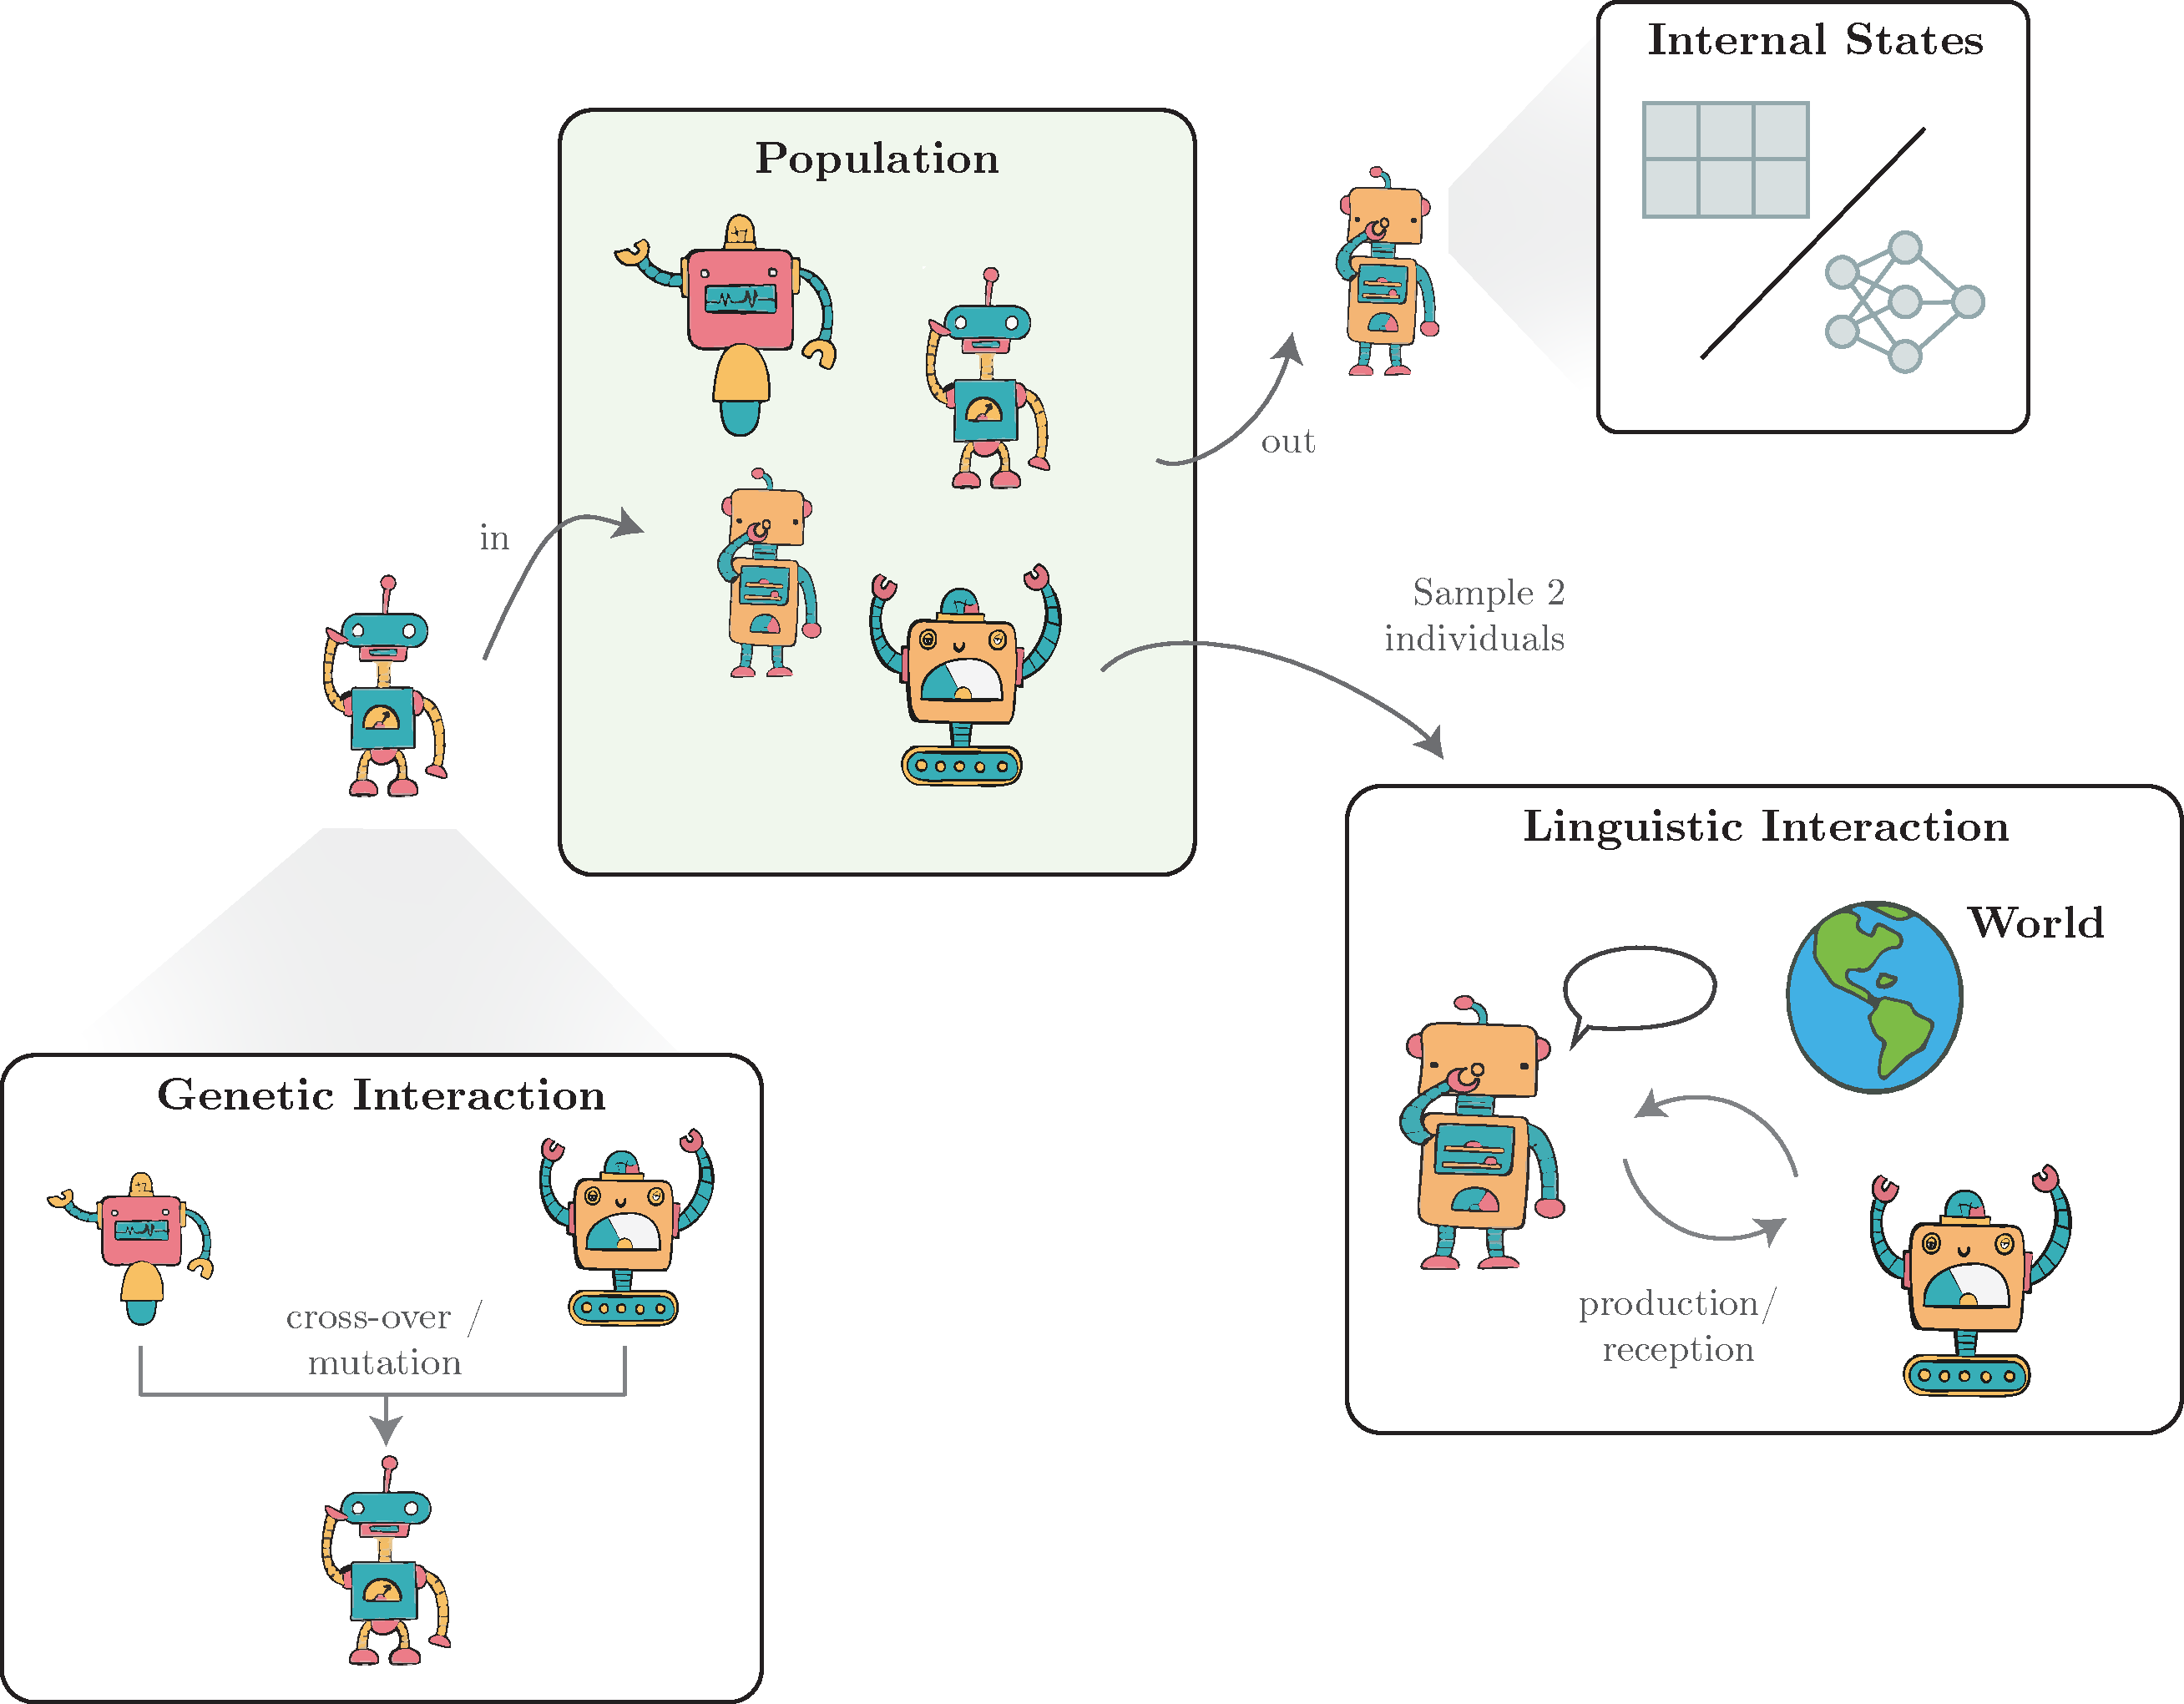
\includegraphics[width=.85\textwidth]{problem_def/language_acquisition_framework.pdf}	
\caption{The Language formation framework: A population of agents is an open multi-agent system where new agent enters and others leave. New agents are generated by genetic interactions: crossovers between parents with potential mutations. Agents have internal states allowing them to map signals to actions. They can perform linguistic interactions, i.e. exchanging messages to describe a physical situation of the world.}
\label{fig:language_acquisition_framework}
\end{figure}
%
\begin{algorithm}[!h]
    \begin{algorithmic}
    \small
        \caption{\label{alg:langage-acquisition}Language formation Simulation}
        \REQUIRE Language Interaction $L$, Genetic Interaction $G$, Environment $\mathcal{E}$
        \STATE \textbf{Initialize} Population $\mathcal{P}_A$ and internal states of agents 
		\LOOP
        \STATE Sample two agents from population: $(A_1,A_2) \sim \mathcal{P}_A$ 
        \STATE Store result of linguistic interaction about the world: $ \leftarrow L(A_1,A_2,\mathcal{E})$
        \STATE Update $A_1$ and $A_2$ based on score $s$
        \STATE \textbf{With prob $p_{\text{out}}$:}
        \bindent
        \STATE Remove agent from population: $\mathcal{P}_A$.pop()
        \eindent
        \STATE \textbf{With prob $p_{\text{in}}$:}
        \bindent
        \STATE Sample two parents from population: $(A_1,A_2) \sim \mathcal{P}_A$  
        \STATE Perform Genetic Interaction: $A' \leftarrow G(A_1,A_2)$
        \STATE Add child to population: $\mathcal{P}_A$.add($A'$)
        \eindent
        \ENDLOOP
    \end{algorithmic}
\end{algorithm}

This study will not investigate the impact of population dynamics on the emergence of language. Rather, it will focus on the development of agents during a lifetime and disregard any genetic interactions. We will thus focus on the self-organization of cultural conventions during linguistic interactions. We will restrict our analysis to the smallest population of two individuals. 

\newpage
\paragraph{Language Games}

The simplest forms of linguistic interaction are coined language games. They derive from \textit{Signaling Games} introduced by \citet{Lewis1969} as a game theoretic approach to the problem of the emergence of conventions. In game theoretic words, a convention is a system of arbitrary rules that enables two players to share meaningful information.  \fig{fig:lewis_game} presents a simple example of a Lewis game. The two players of a signaling game are the speaker and the listener. In our example, the world is providing two world states to the speaker ($w_1$ and $w_2$). Based on the world state, the speaker sends a signal to the listener. Here, there are two available signals ($s_1$ and $s_2$). From the received signal, the listener then chose an action (among two actions $a_1$ and $a_2$). If the listener picks the correct action for the associated word state then both agents perceive a reward. Note that the Listener never perceives the world state.  
\begin{figure}[!h]
\centering
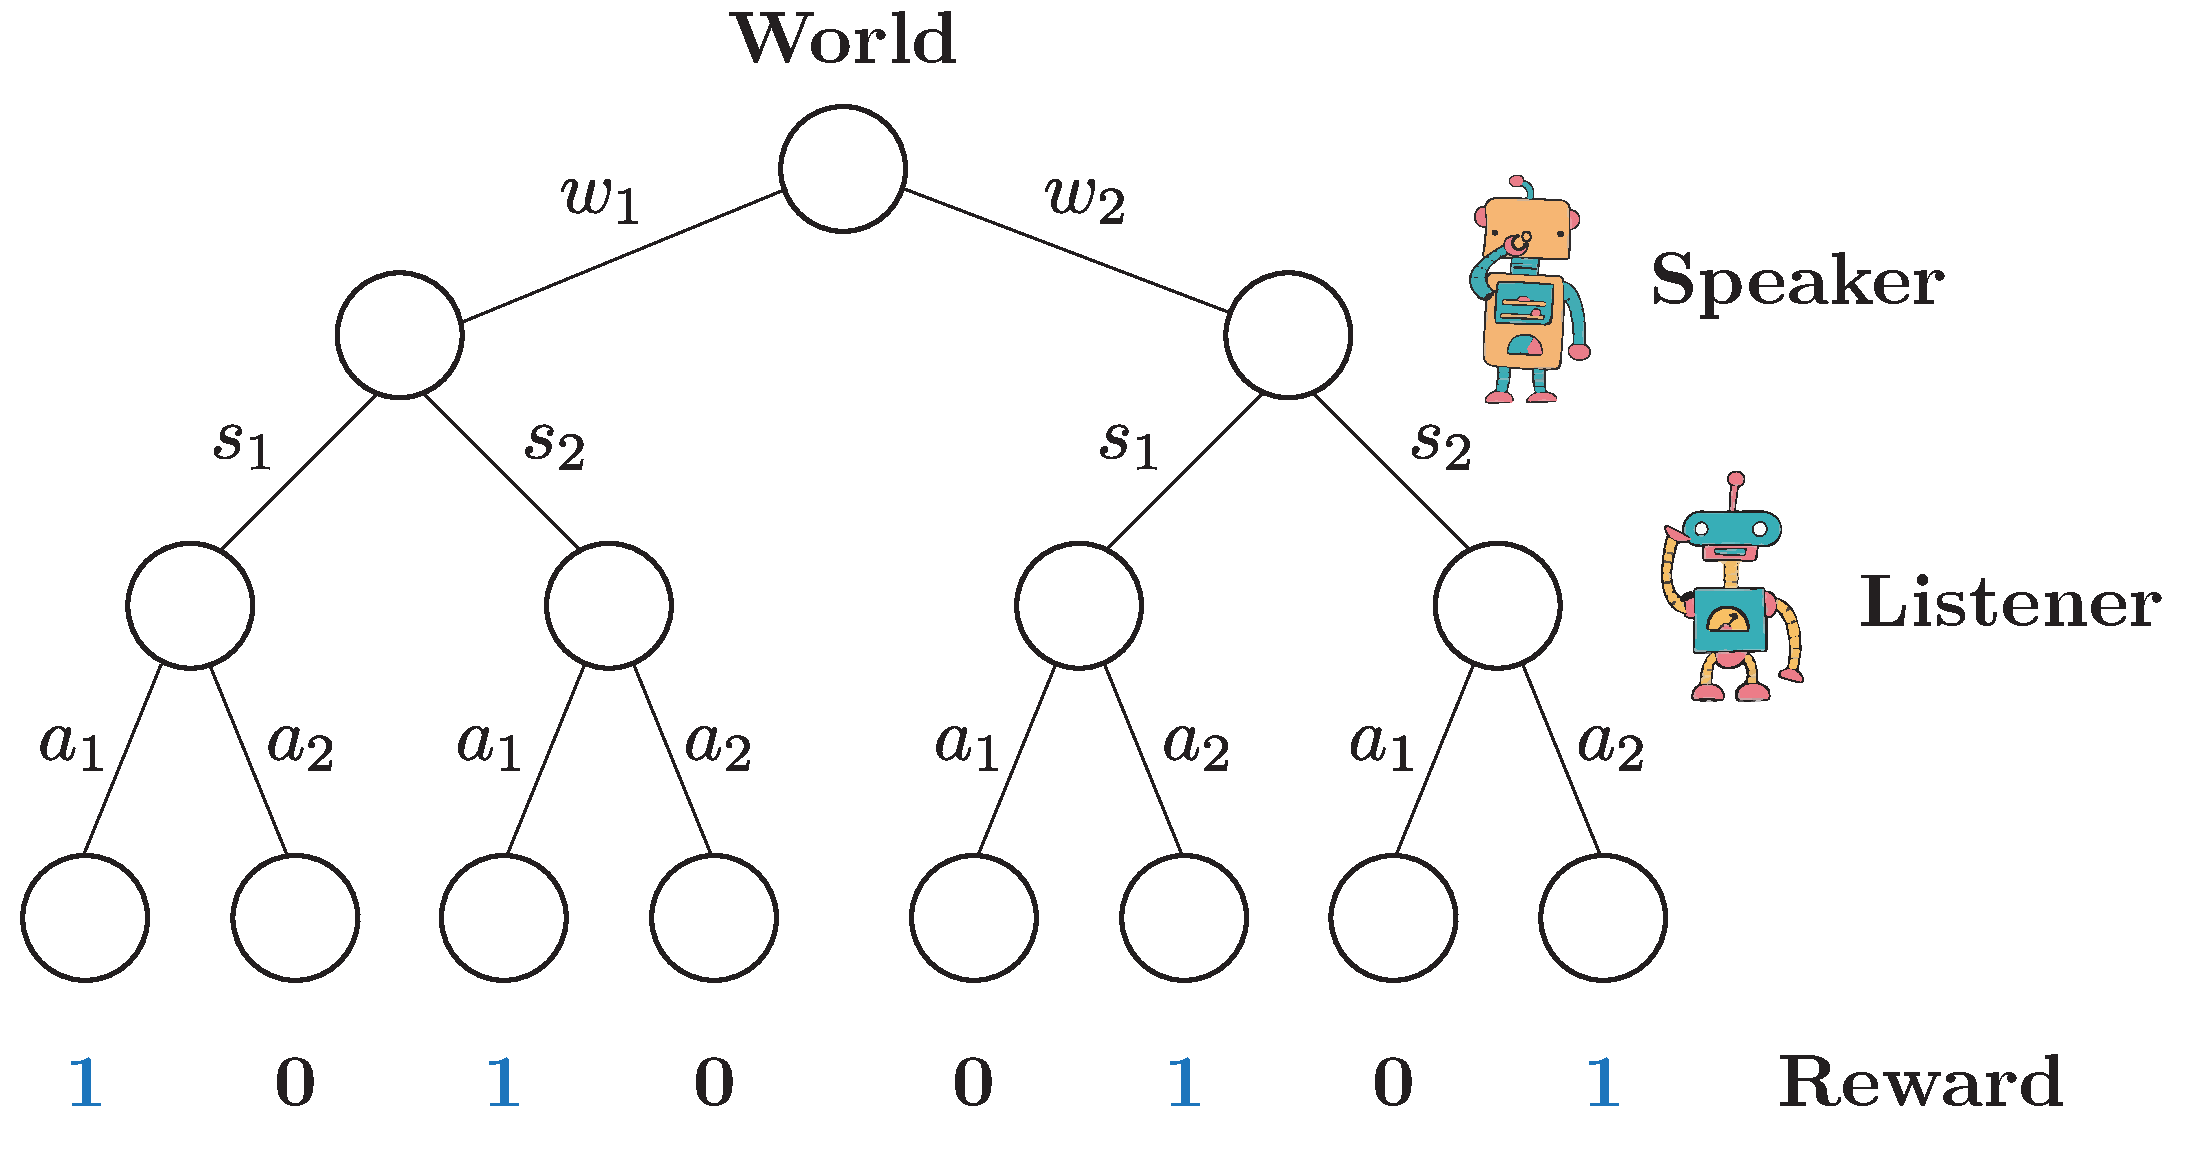
\includegraphics[width=.525\textwidth]{problem_def/lewis_game.pdf}
\caption{Illustration of Lewis Signalling game with two world states, two signs, and two actions.}
\label{fig:lewis_game}
\end{figure}

To investigate the self-organization of conventions around meanings in a more realistic scenario, \citet{steels2012grounded} proposed to update signaling games with grounding elements.  In a grounded language game, the speaker and the listener are given a shared \textit{context} made of several \textit{referents} (objects) as displayed in \fig{fig:language_game_interactions}. The speaker samples a target referent from the context and produces an utterance to name it. Then, the speaker receives the utterance and picks a referent inside the context. If the chosen referent matches the target referent, the game is a success. To self-organize a language, a population of artificial agents needs to play numerous language games. In doing so, agents will alternate between speakers and listers. Depending on the outcome of the game they will update their internal states to reinforce successful conventions and diminish unsuccessful ones. Note that several update strategies are possible. They vary in how the outcome is actually perceived by the agents. On the speaker side, the referent ground truth (target) is known so the outcome of the game can be directly used for the update. On the other hand, since the listener does not know about the target referent some implementations of language games do not communicate the outcome to the listener. In \citet{steels2001language}'s formulation of language game, the outcome is communicated to the speaker via a retroactive pointing mechanism. The speaker basically points toward the target referent at the end of the game to communicate the outcome to the speaker.

\begin{figure}[!h]
\centering
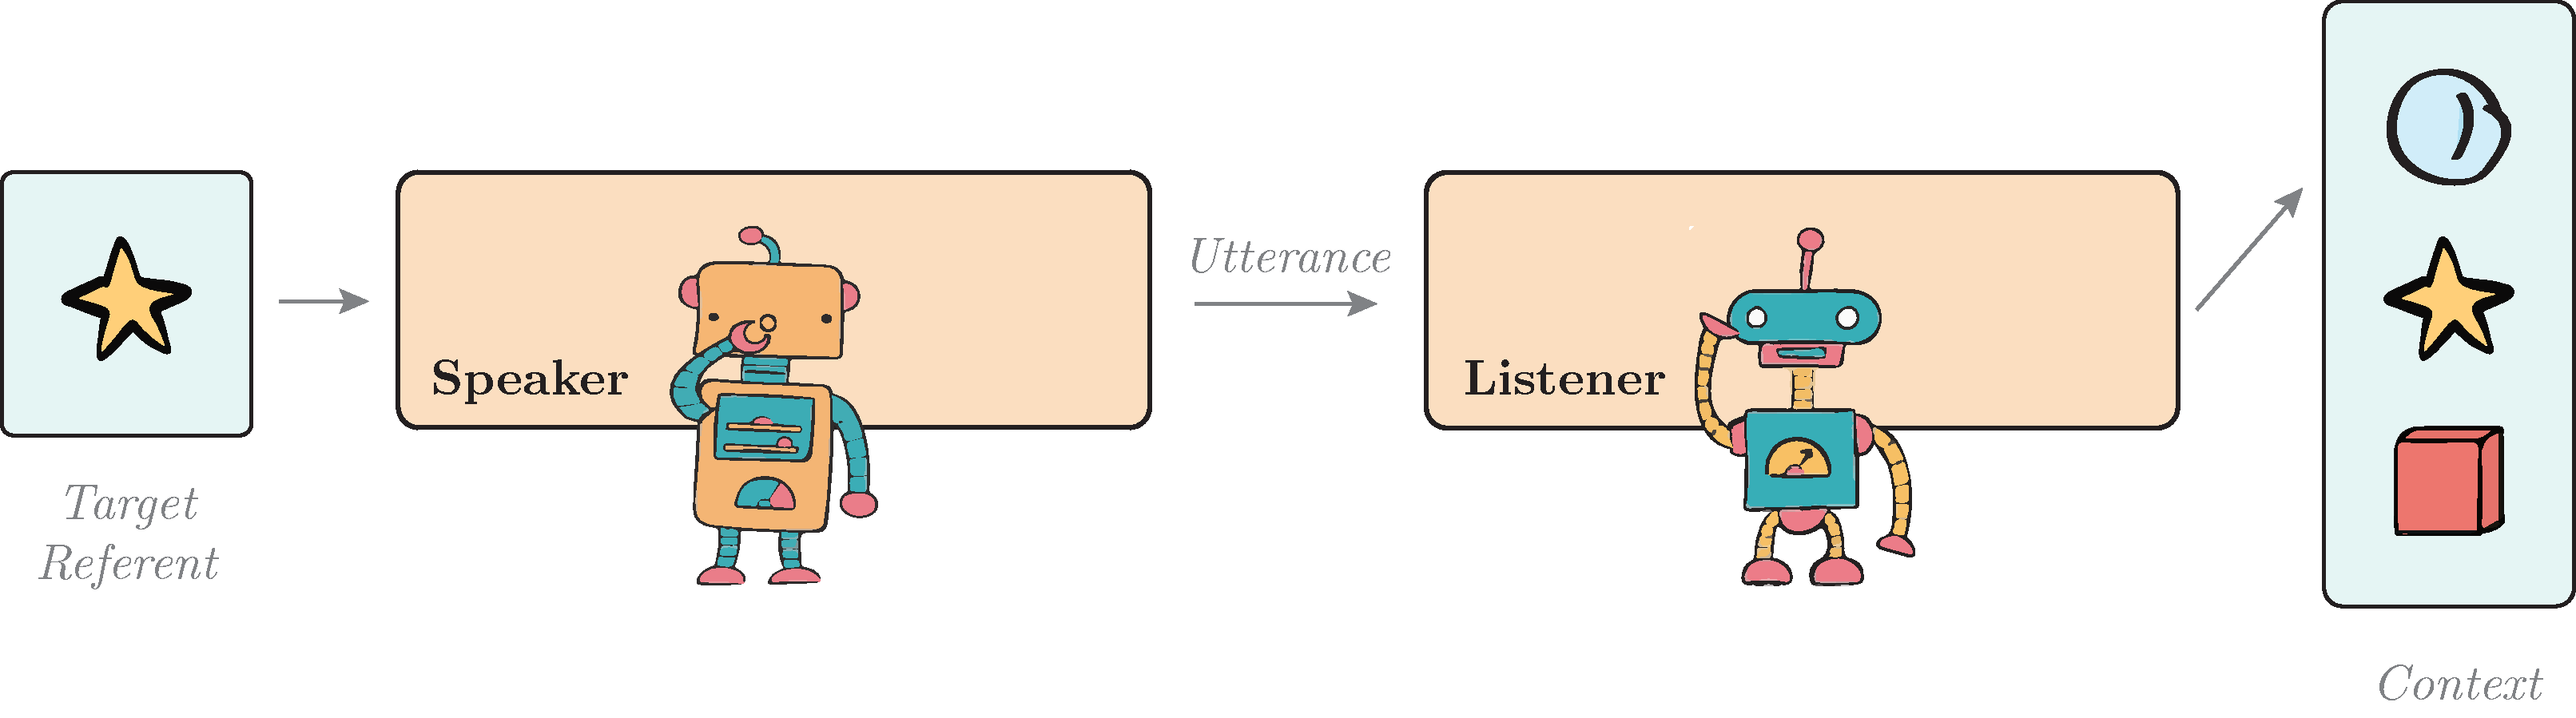
\includegraphics[width=.8\textwidth]{problem_def/language_game_interactions.pdf}	
\caption{Diagram of interactions in a language game}
\label{fig:language_game_interactions}
\end{figure}

Early solutions to the language game~\citep{steels1995selforganizing,batali1997learning,kirby2001spontaneous} use tables scoring associations between referents and utterances. Given fixed predefined numbers of utterances and referent categories, the agents can adjust the score of utterance/referent association depending on their communicative success. Examples of such tables for the speaker (left) and for the listener (right) are given in \fig{fig:language_game_tabular}.  If predefined referent categories are not available to the agents, \citet{steels2012grounded} propose mechanisms to map visual inputs to object categories. Similarly, the Talking Head experiments~\citep{steels2015talkingheads} propose strategies to adapt the language game to more realistic configurations with flexible and dynamic inventories of words and meanings.

\begin{figure}[!h]
\centering
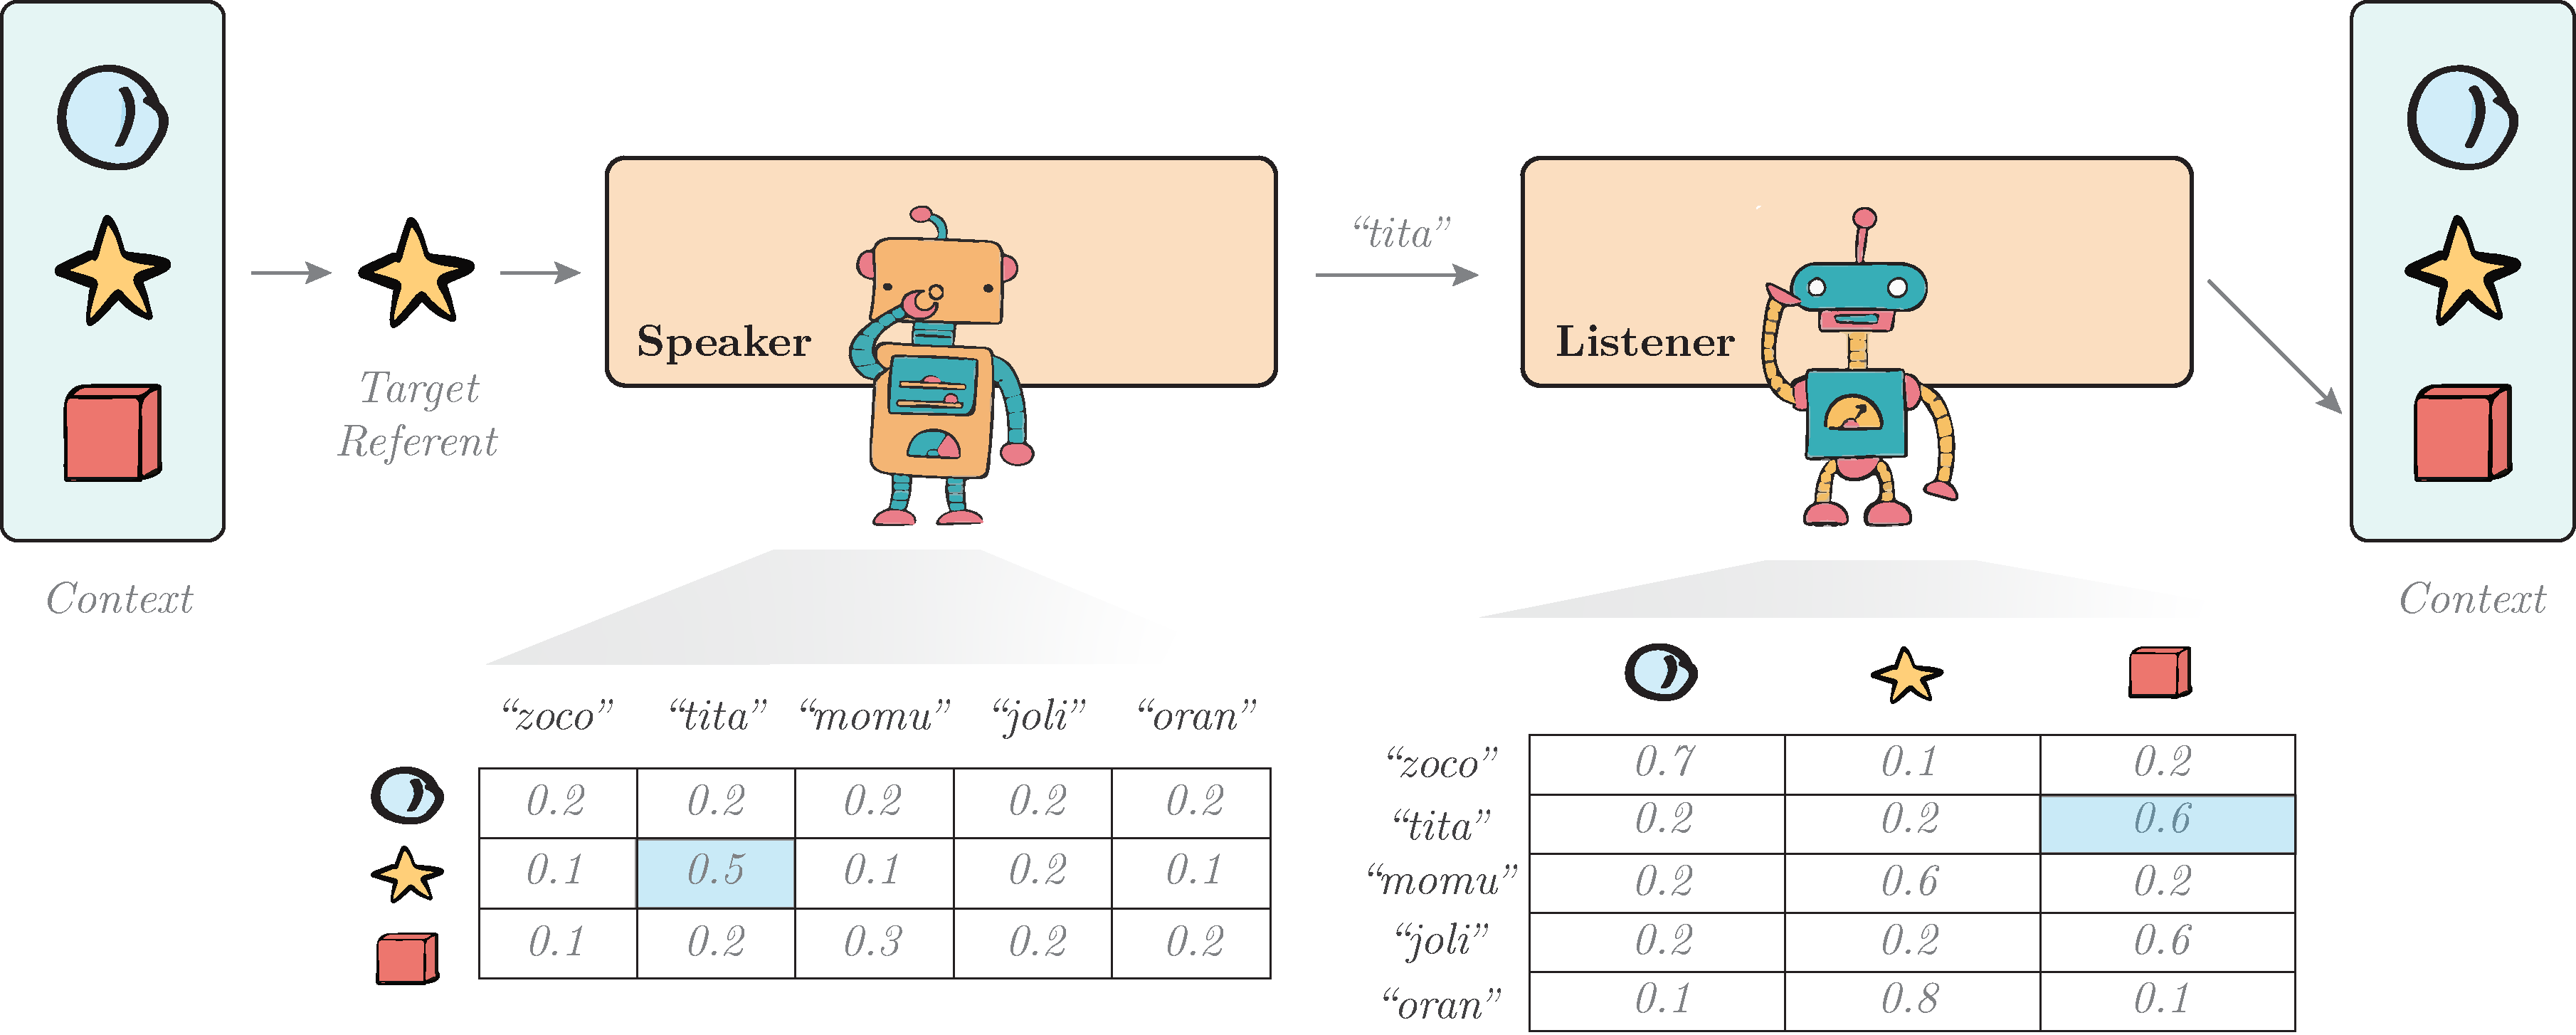
\includegraphics[width=.8\textwidth]{problem_def/language_game_tabular.pdf}	
\caption{Example of agents' tabular internal models, with 3 referents and 5 words.}
\label{fig:language_game_tabular}
\end{figure}

\paragraph{Neural Communicating Agents}

Inspired by the success of Convolutional Neural Network in Computer Vision, \citet{lazaridou2017multiagent} proposed to extend language games to image referents with agents using neural networks to take actions \footnote{In deep learning, language games are often referred to as referential games or guessing games}. \fig{fig:language_game_network} illustrates their setup. The context is made of two images ($i_1$ and $i_2$), a target ($t$) and a distractor. The utterances are discrete utternaces $u$ coming from a fixed-sized dictionary $\mathcal{V}$.  The speaker's utterance is given by a neural network parametrizing a policy that maps the two images to the utterance: $u=\pi_S(i_1,i_2,t; \theta_S)$. Similarly, the listener uses policy $\pi_L$ to make a choice given the utterance: $a=\pi_L(i_1,i_2,\pi_S(i_1,i_2,t; \theta_S);\theta_L)$. The policies are trained using \rl (\sect{sec:background_rl}) with reward function $R$ returning 1 iff $\pi_L(i_1,i_2,\pi_S(i_1,i_2,t; \theta_S);\theta_L) := t$. Note that in their implementation the reward and thus the outcome of the game is communicated to both agents which is equivalent to Steel's pointing mechanism. 

\begin{figure}[!h]
\centering
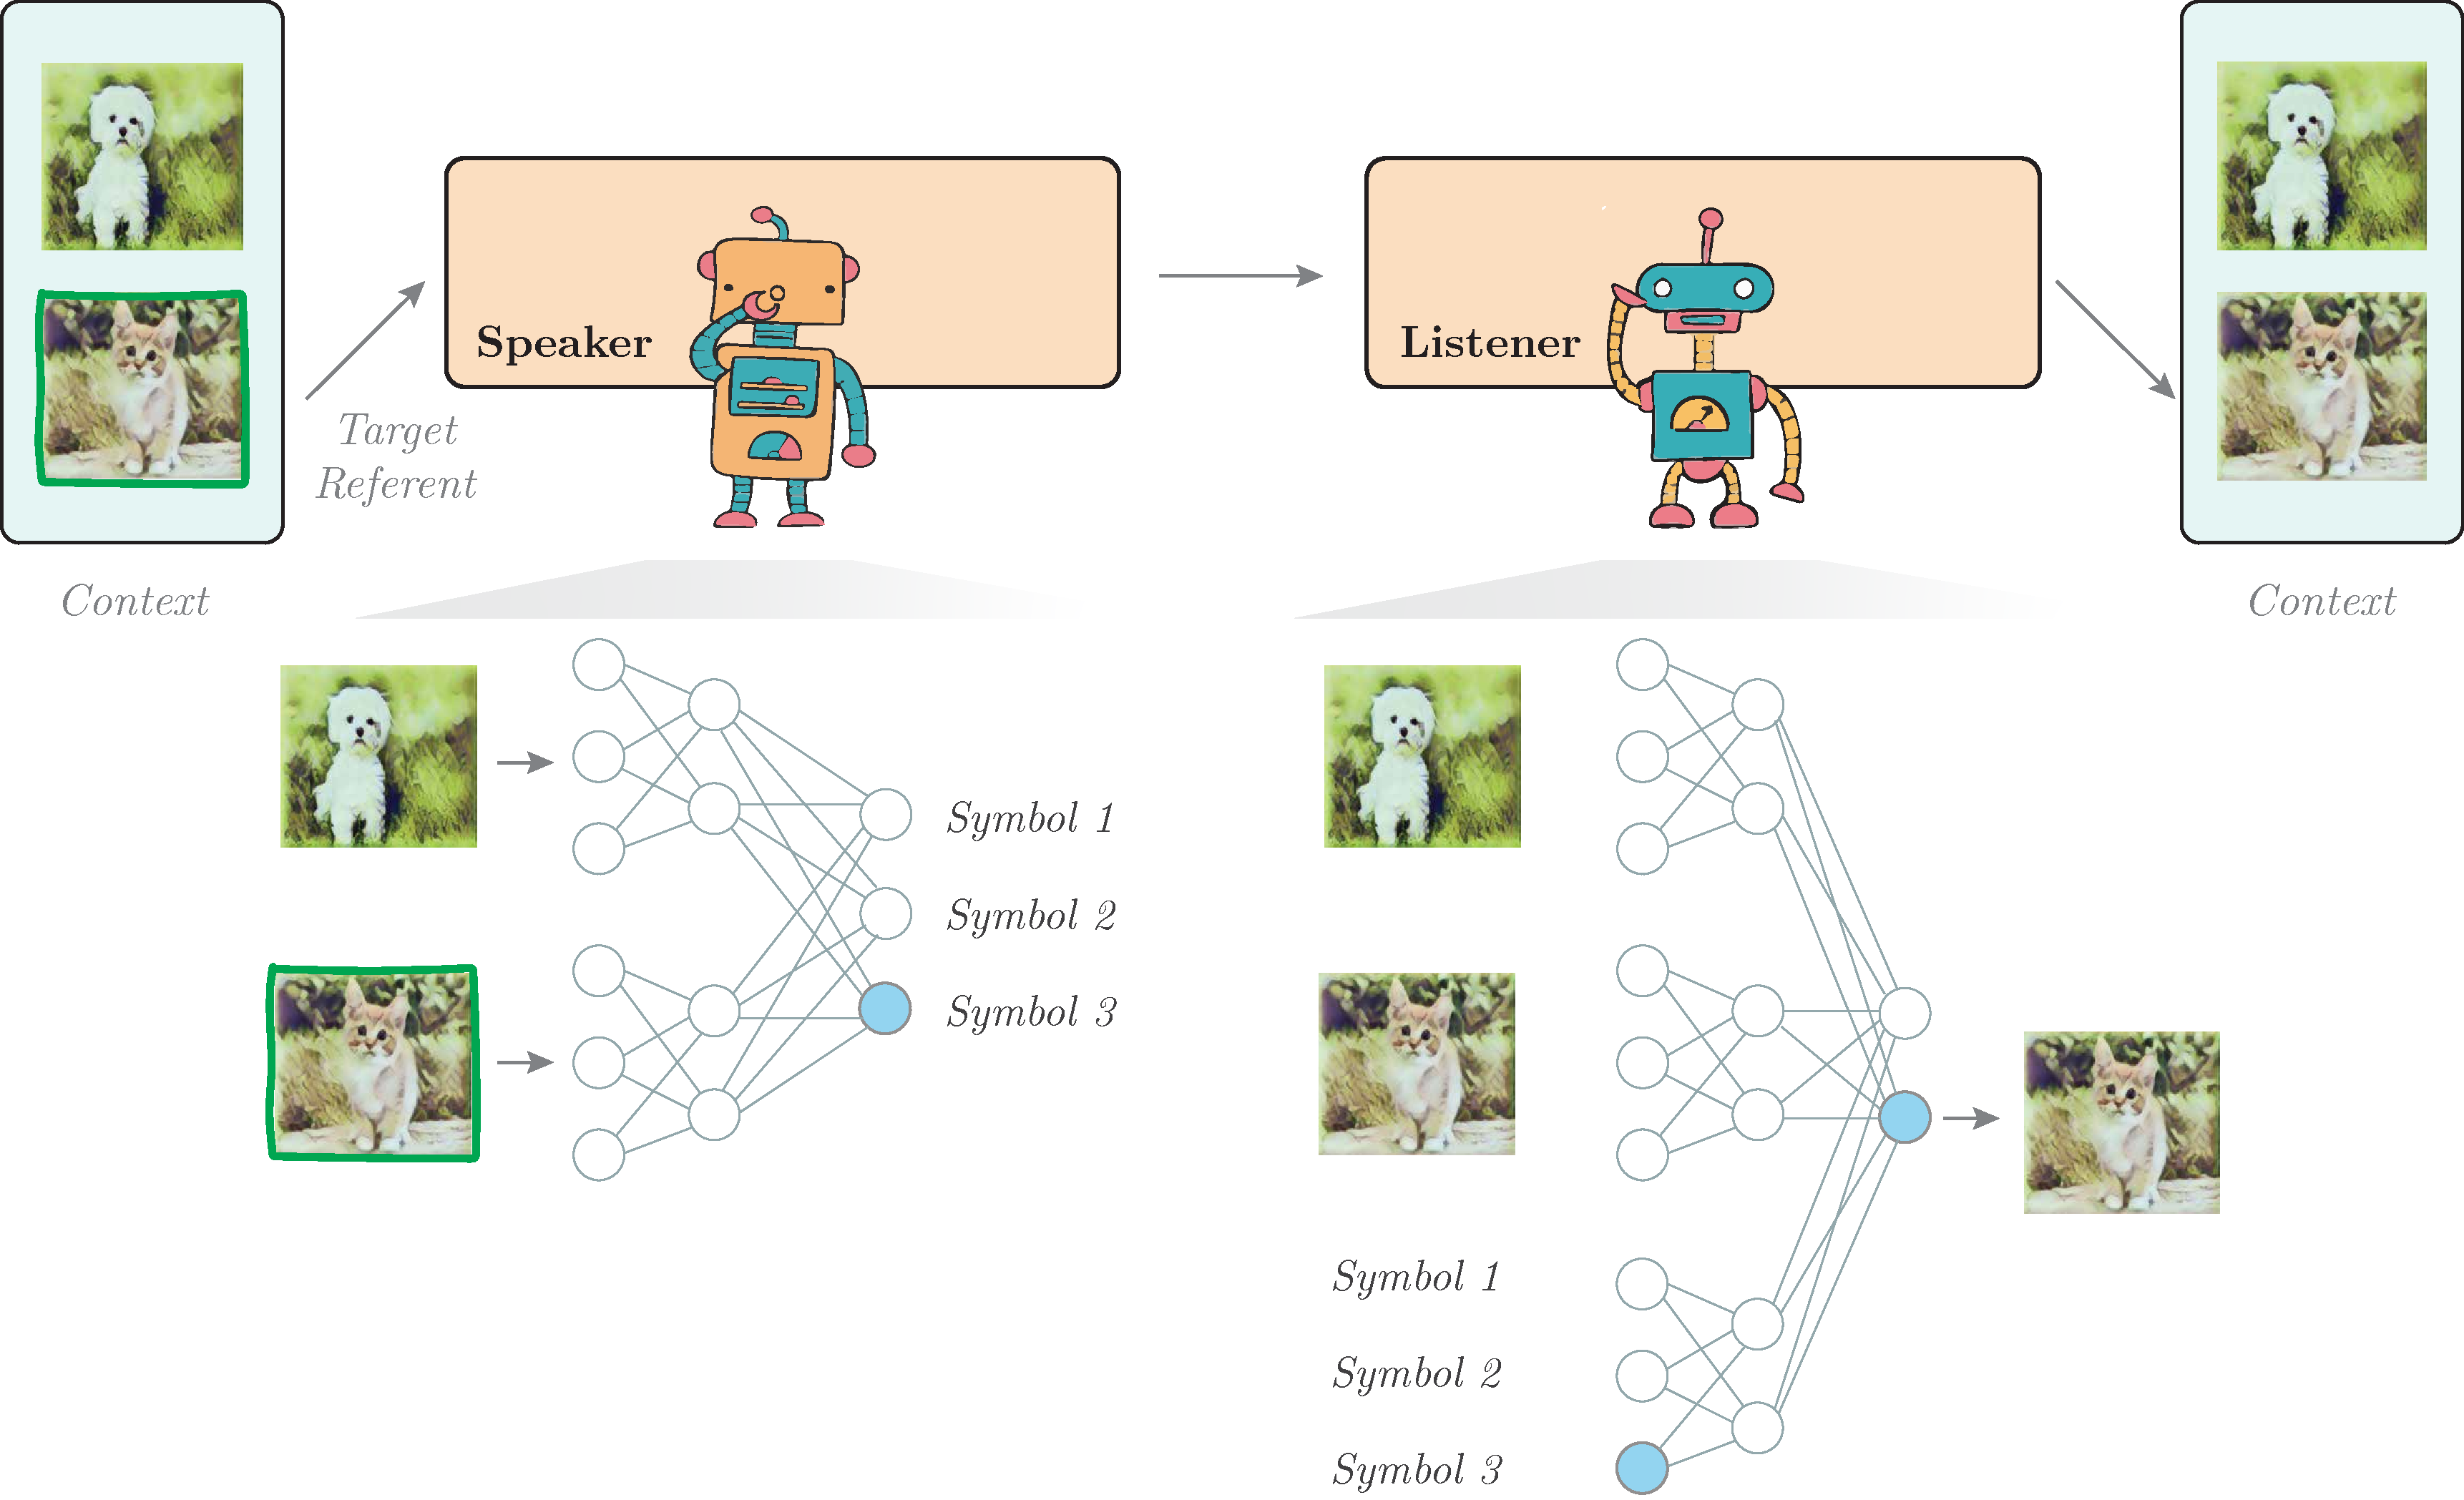
\includegraphics[width=.8\textwidth]{problem_def/language_game_network.pdf}	
\caption{Example of agents' neural network internal models, with 2 referents and 3 words (adapted from \citet{lazaridou2017multiagent}).}
\label{fig:language_game_network}
\end{figure}

Beyond scaling previous language game approaches to visual referents, \citet{lazaridou2017multiagent} proposes a strategy to ground the agent's code in natural language. The strategy consists in leveraging a dataset of (image, natural language label) pairs and alternating between \rl in the classical language game and standard supervised learning for image classification. In a similar study, \citet{havrylov2017emergence} examine the emergence of communication with sequences of symbols and visual referents. They use \lstms within the speaker and listener architectures to support the encoding and decoding of discrete tokens arranged in fixed-size sequences. They also analyze the compositionality and variability of the emerging sequences in both tabular-rasa and natural language communication. 

The identification of the factors that contribute to the emergence of compositional communication code is a fundamental objective within the field of computational linguistics. To this end, the use of neural communicating agents in language games has emerged as a valuable experimental setting. \citet{kottur2017natural} propose to analyze how utterances consisting of sequences of symbols can name referents that are compositions of abstract attributes (represented as one-hot vectors). The decomposition of referents into pre-defined hardcoded attributes enables a more comprehensive and systematic analysis of the compositional properties of the evolving communication code. Building upon this work, \citet{chaabouni2020compositionality} emphasize the importance of separating the compositional generalization capabilities of agents and compositional properties of the emerging code. They have established that the former can be achieved independently of the latter. Other works look at the environmental and internal factors that favor the emergence of compositionality. For instance, \citet{rodriguez-luna-etal-2020-internal} show that auxiliary objectives incentivizing object consistency or least effort (the generation of short sequences) support the emergence of compositional code in language games. Similarly, \citet{mu2021emergent} demonstrate that agents solving a variation of the language games where referents are organized in sets of objects agree on a more interpretable and systematic communication code. Finally, \citet{Ren2020Compositional} proposed to study the emergence of compositional code in a more complete setting with a population of agents playing language games over several generations.

\paragraph{Goal-Directed Communicating agents}

The prior paragraph demonstrates that guessing interactions provide an effective experimental testbed to study Language formation. But, as outlined in the introduction, human language serves a multitude of purposes beyond mere object guessing. Therefore, \ai researchers have aimed to examine the development of communication in more realistic scenarios, where agents must communicate to accomplish a collaborative task in complex environments that involve interactions with the physical world across multiple time steps. These problems are modeled using \marl as described in \sect{sec:background_marl}. The agents must concurrently learn to interact with the world and communicate with others by observing rewards related to their collaborative goal, provided by an expert. See \fig{fig:marl_comm_interactions} for a visual representation of these interactions. Seminal works on \marl involving communicating agents consider problems such as efficient car coordination at traffic junctions to avoid collision~\citep{sukhbaatar2016learning} or riddles where agents need to combine environmental inputs with information communicated over several time steps to succed~\citep{foerster2016learning}. In their work, \citet{foerster2016learning} introduce two approaches for learning to communicate in \marl: Differentiable Inter-Agent Learning (\textsc{dial}) and Reinforced Inter-Agent Learning (\textsc{rial}). \textsc{dial} is based on the centralized training and decentralized execution method and enables gradient to be exchanged between agents, thereby breaking the assumption of the Language formation framework that agents should not be able to have access to each other's internal states. Conversely, in \textsc{rial}, messages are viewed as actions produced by a \rl algorithm where each agent treats others as a part of the environment, without the need to have access to other agents’ internal parameters or to back-propagate gradients. The \textsc{rial} algorithm now serves as a baseline for a variety of \marl communication investigations. \cite{jiang2018learning} extended it with an attention mechanism that enables agents to learn when communication is required to solve collaborative tasks.  Similarly, \citet{eccles2019biases} showed that adding positive signaling (messages must be different in different situations) and positive listening (actions must be different when messages are different) biases to agents via auxiliary losses yields an increase in communicative performance. For a complete survey of emergent communication in \marl setups, see \citet{zhu2022survey}.

\begin{figure}[!h]
\centering
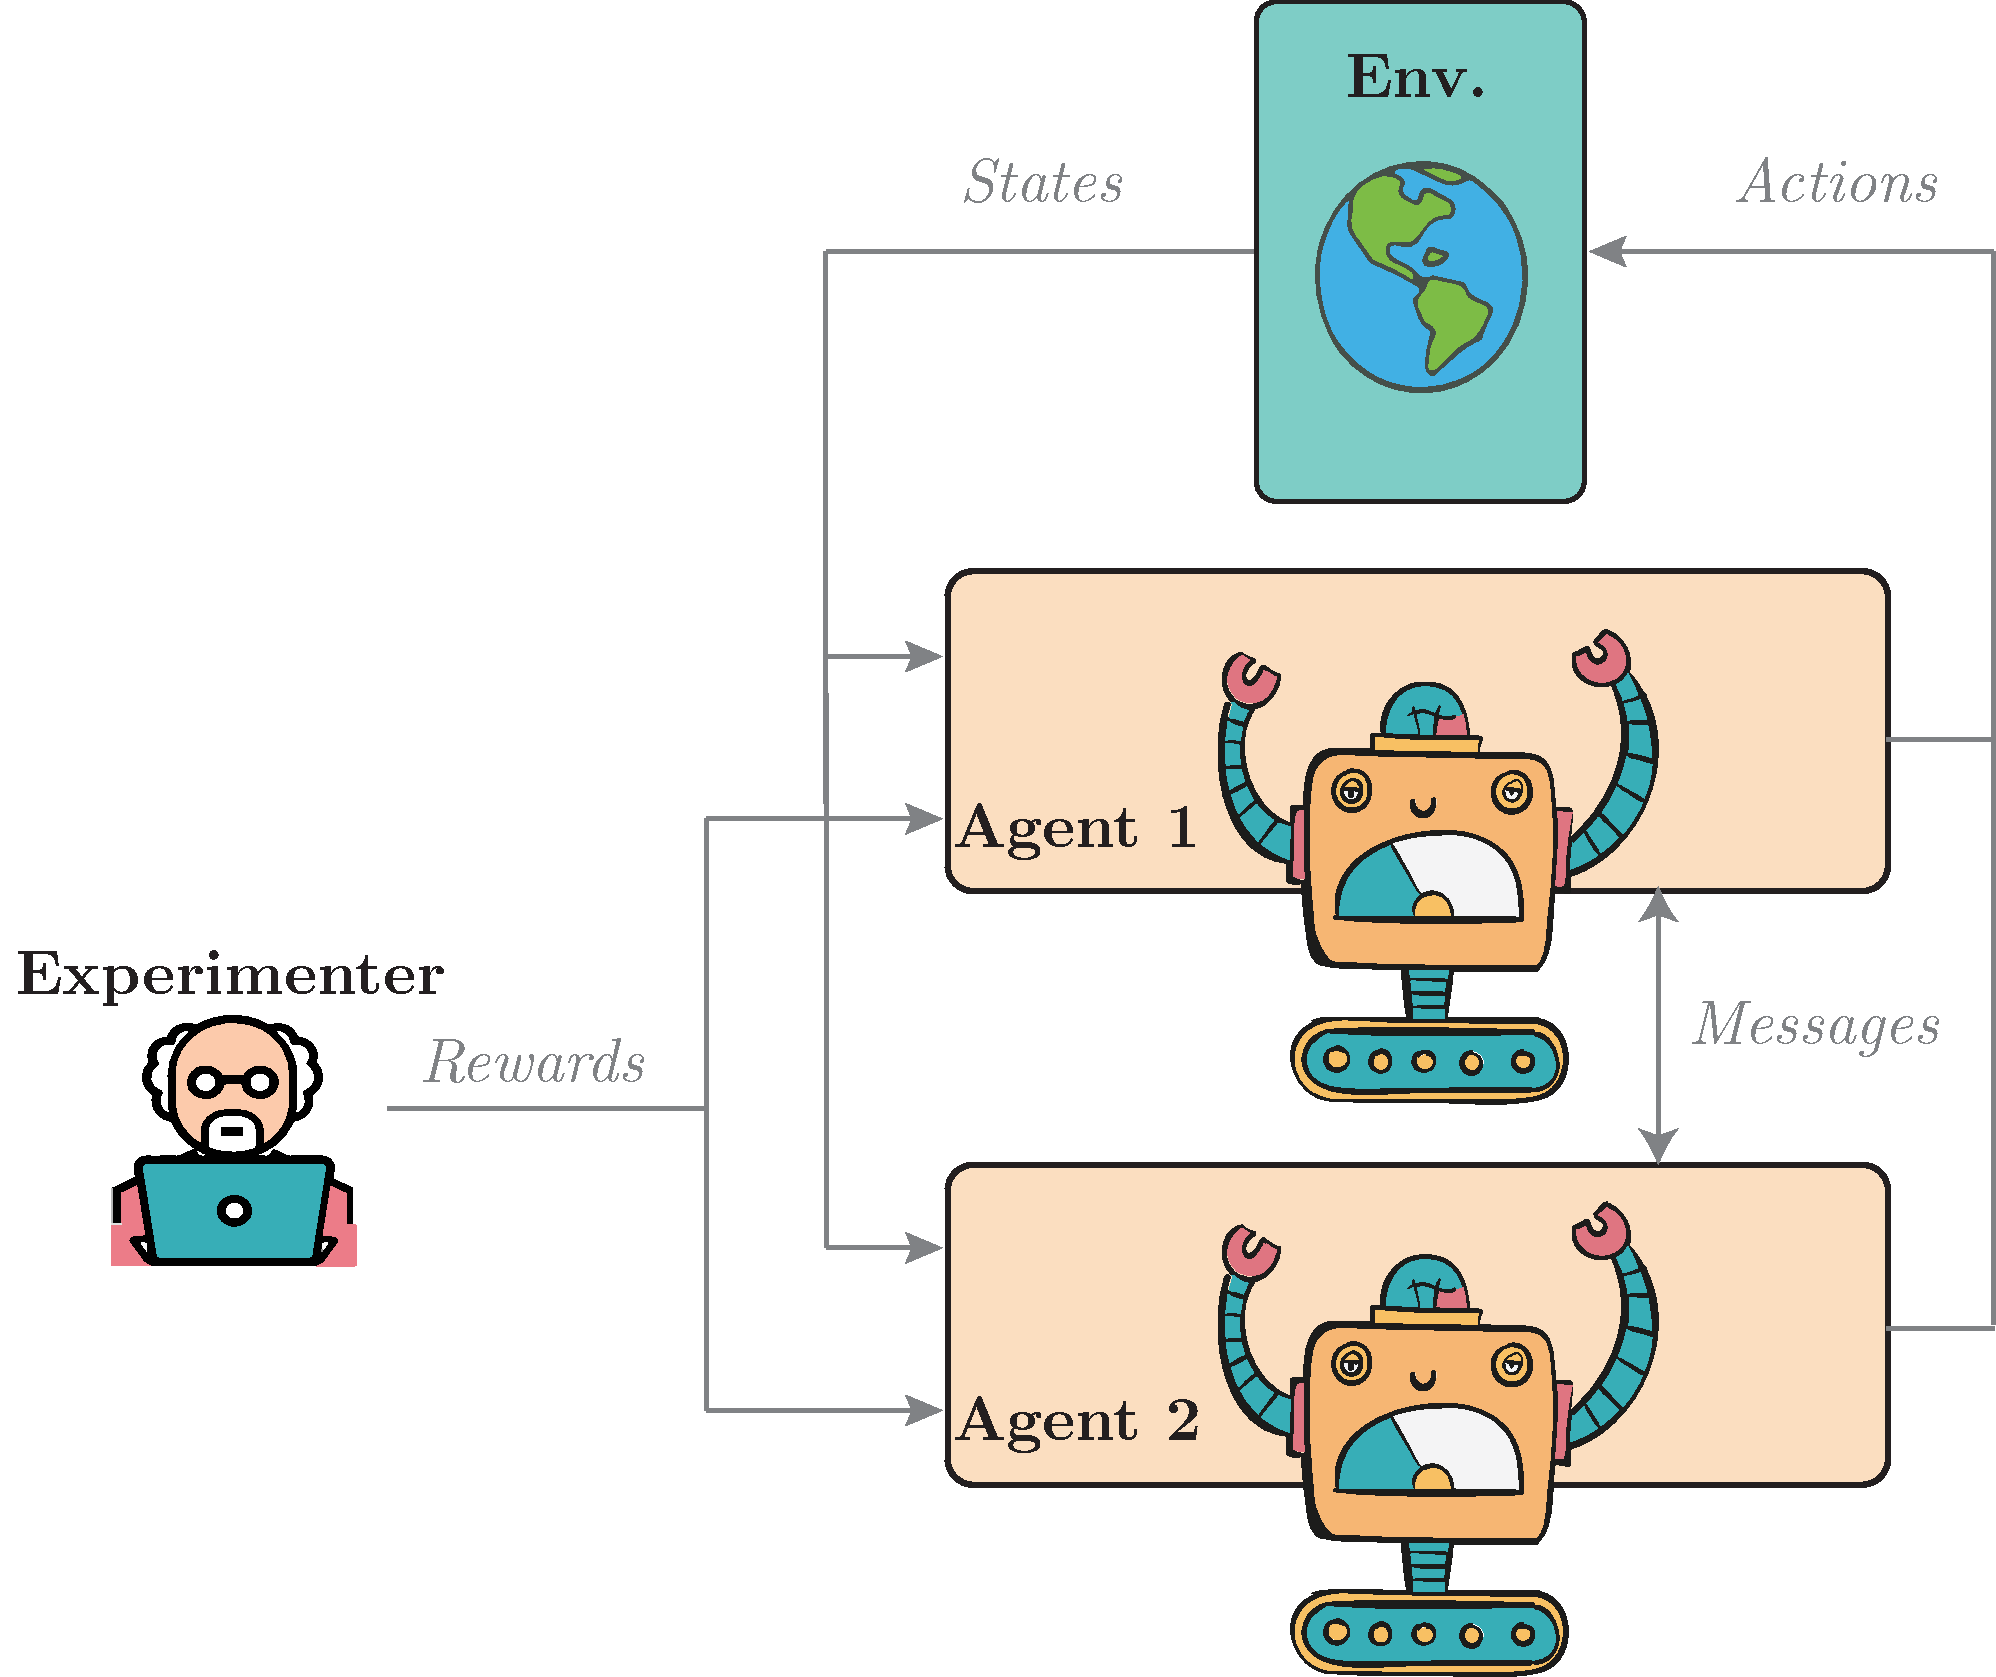
\includegraphics[width=.5\textwidth]{problem_def/marl_comm_interactions.pdf}	
\caption{Diagram of interactions in \marl emergence communication.}
\label{fig:marl_comm_interactions}
\end{figure}


\paragraph{Summary}

In this section, we presented the Language formation framework which study the emergence of communication inside a population of agents interacting within linguistic and genetic interactions. Our contributions focus on linguistic interactions and ignore the influence of population dynamics on the emergence of communication. We, therefore, presented the most broadly studied linguistic interactions: the language game. Additionally, we showed that this particular guessing interaction setup could be scaled to neural agents. Finally, we noted that \marl offers a valuable framework to study the emergence of communication as a tool to achieve collaborative behaviors in physically complex environments. 

\subsection{Problem Definition}

\label{sec:self-orga-lang-prob-def}

It this now time to turn to our contributions and to formally pose the specific inquiries we target within the context of artificial communicating agents.

\paragraph{Emergence of Graphical Sensory-motor Communication}

 Our first contribution \todo{add chapter ref}  extends the neural communicating agent framework to consider communication in visual language games via a sensory-motor channel. As reviewed in the previous section, prior approaches focused on agents communicating via an idealized communication channel, where utterances (made of a single or a sequence of symbols) are produced by a speaker and directly perceived by a listener. This comes in contrast with human communication, which instead relies on a \emph{sensory-motor channel}, where motor commands produced by the speaker (e.g. vocal or gestural articulators) result in sensory effects perceived by the listener (e.g. audio or visual).  Motivated by this observation we investigate whether artificial agents can develop a shared language in an ecological setting where communication relies on such sensory-motor constraints. To this end, we introduce the \textit{Graphical Referential Game}(\greg) where a speaker must produce a graphical utterance to name a visual referent object while a listener has to select the corresponding object among distractor referents, given the delivered message as illustrated in \fig{fig:prob_def_greg}. The utterances are drawing images produced using dynamical motor primitives combined with a sketching library. The referents are images of MNIST~\citep{LeCun1998GradientbasedLA} digits randomly positioned in the image.  The utilization of sensory-motor systems to examine the development of language dates back to the investigation of the origins of digital vocalization systems in the early 2000s~\cite{deBoer2000selforganization,oudeyer2005selforganization,zuidema2009evolution}. However such studies were not conducted in grounded language games. They employed imitation games focusing on the observation of the formation of speech utterances, such as syllables and words, through the systematic combination of lower-level meaningless elements (phonemes). In our study, we chose to focus on a drawing system because 1) conversely to models of vocalization, there is a large number of tools available to researchers to implement realistic sketching mechanisms and 2) it has the advantage of producing 2D trajectories interpretable by humans while preserving the non-linear properties of speech models, which were shown to ease the discretization of the produced signals~\cite{STEVENS19893,MOULINFRIER20155}.
 
\begin{figure}[!h]
\centering
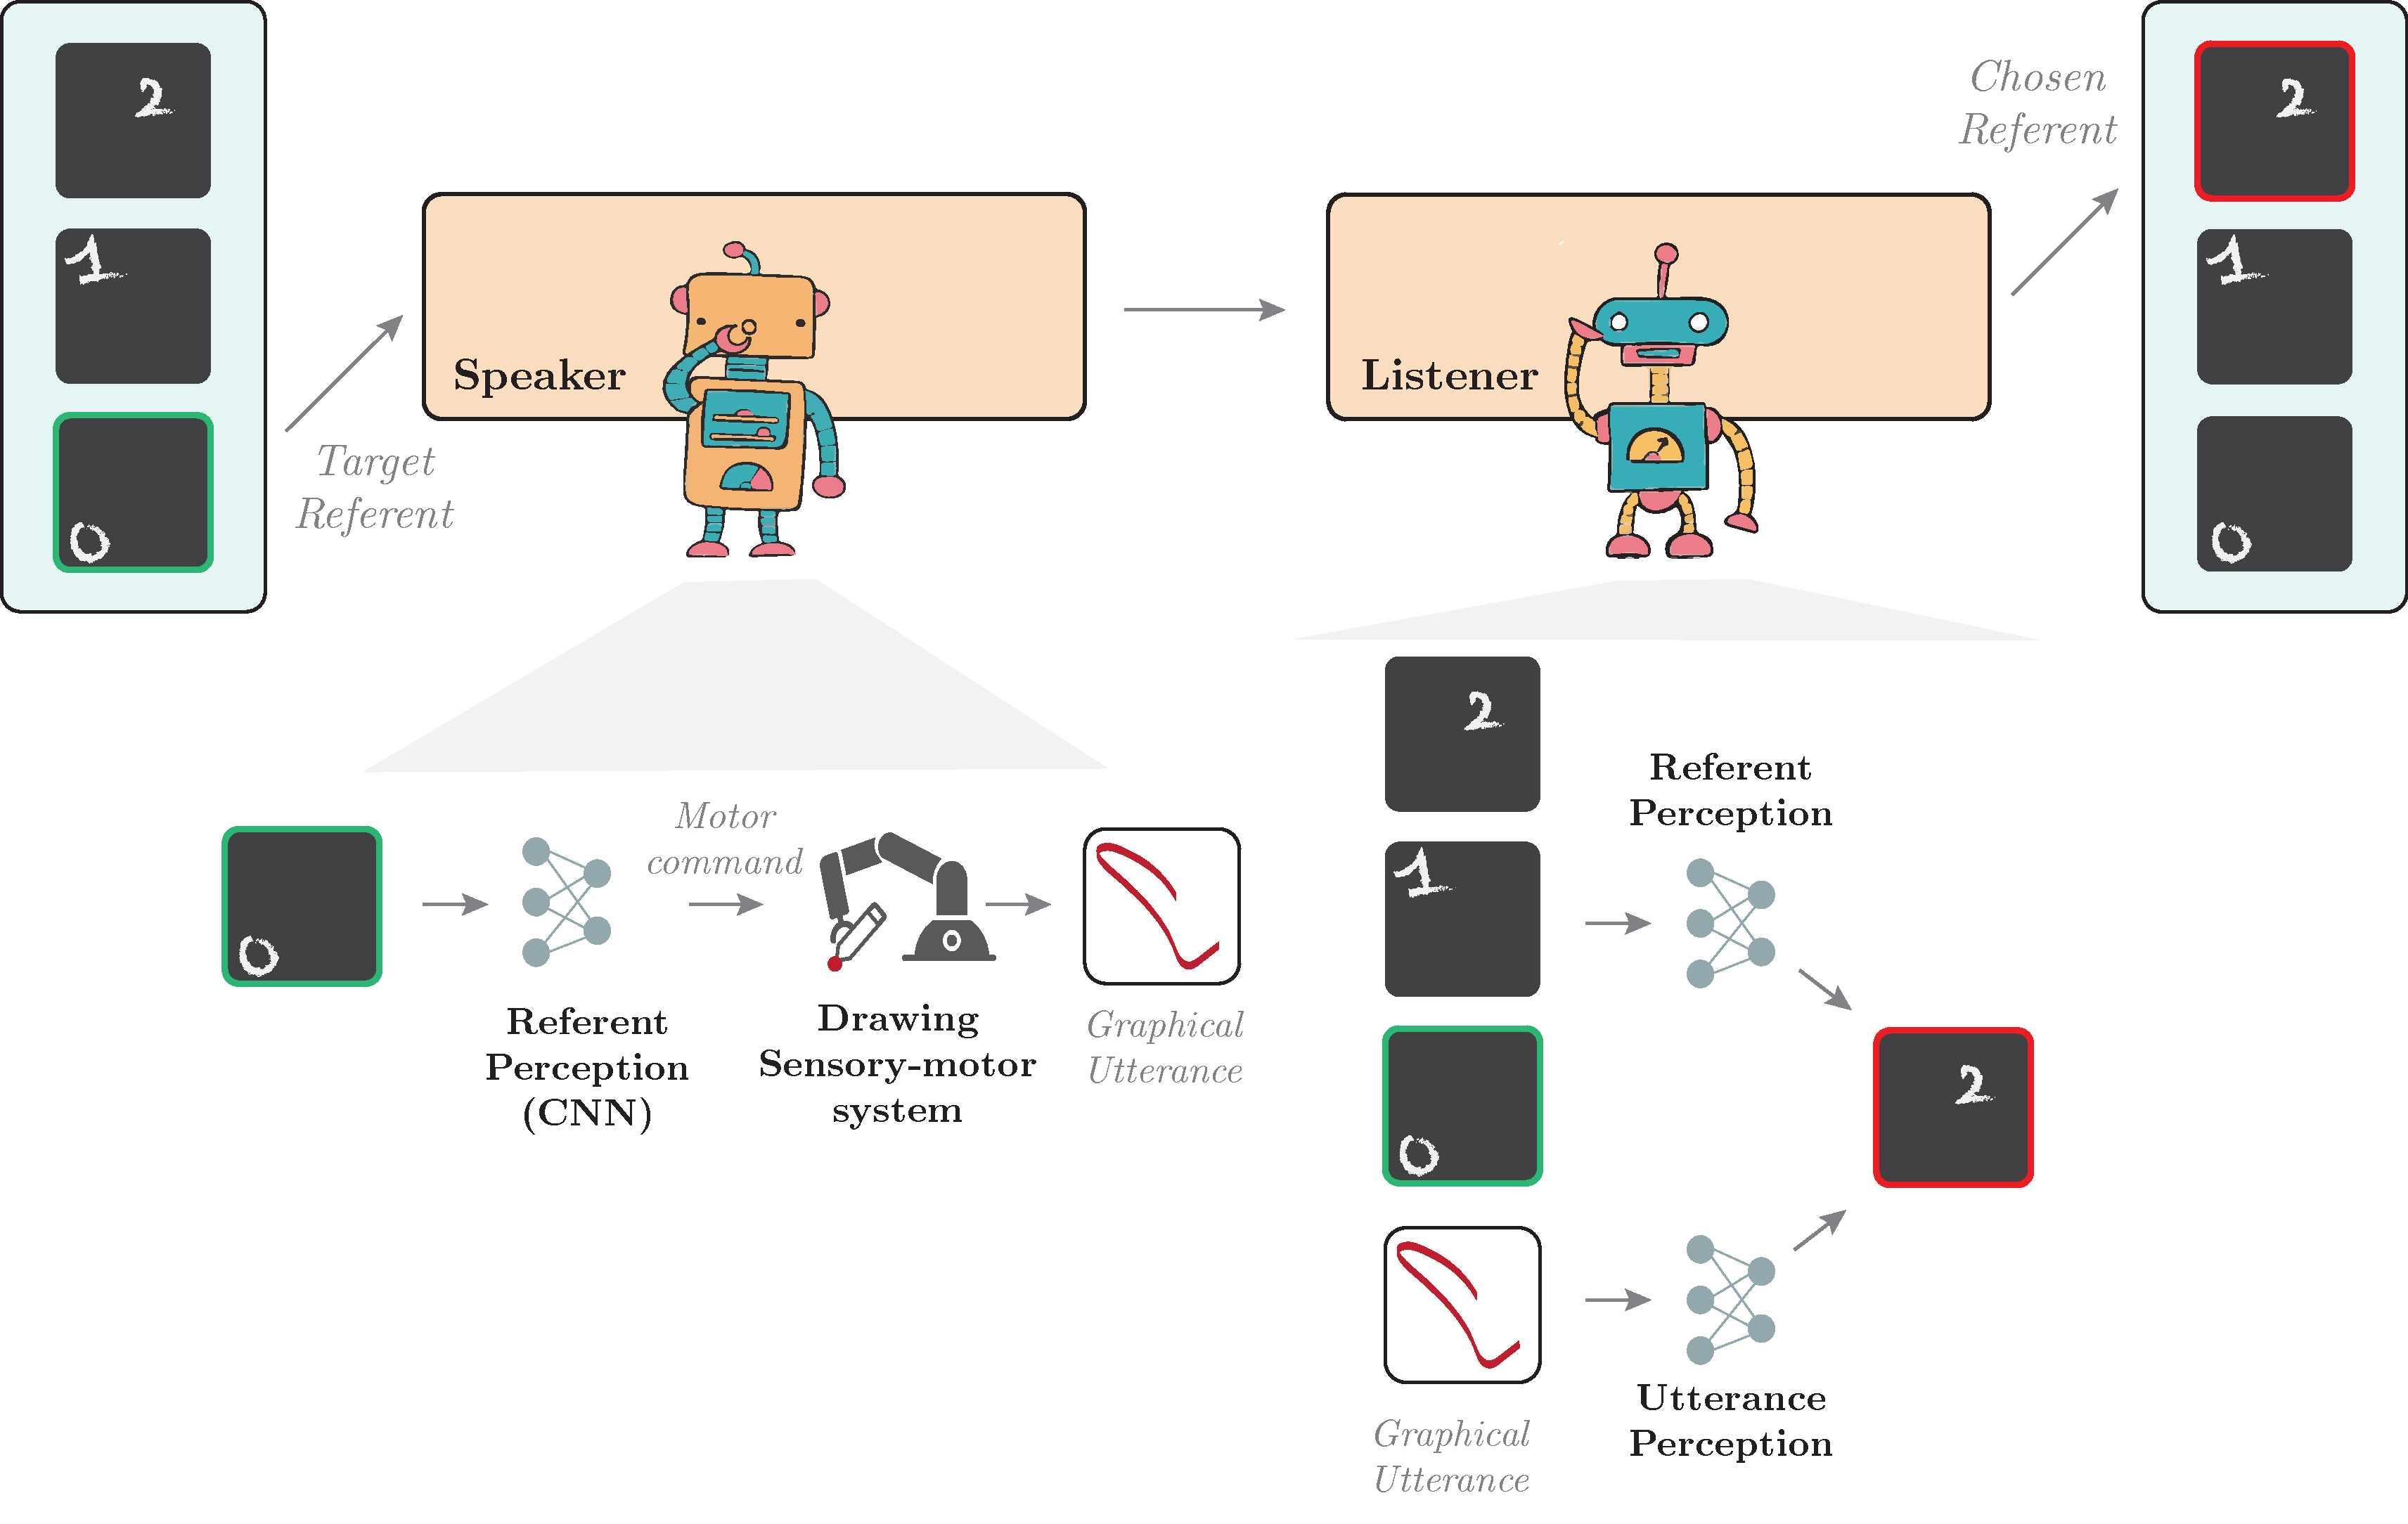
\includegraphics[width=.8\textwidth]{problem_def/prob_def_greg.pdf}	
\caption{The Graphical Referential Game}
\label{fig:prob_def_greg}
\end{figure}

Studying the \greg we aim at investigating whether a pair of agents can self-organize a shared lexicon from the continuous non-linear constraints of the sensory-motor system. We then propose to study the structure of the emerging signals. We use topographic measures based on a geometric distance to quantify the coherence of the emerging lexicon. Informed by \citet{chaabouni2020compositionality}'s study on the non-equivalence between compositional performance and compositional language, we propose to study these two questions separately. More precisely, we evaluate the communicative generalization performances of our system on referents that are the composition of MNIST digits. We end our study investigating the compositional structure of emerging signs using the same geometry measure as for the coherence.

\paragraph{The Architect-Builder Problem}

Our second contribution proposes to study the \textit{Architect-Builder problem} (\abp), a new \ai paradigm that studies the goal-directed emergence of communication in a setup where the reward function is not accessible to all agents. The \abp involves two agents, referred to as the \textit{Architect} and the \textit{Builder}, who must collaborate to accomplish a task. Both agents observe the environment state but only the architect knows the goal at hand. The architect possesses knowledge of the goal and is able to receive the reward associated with it, but is unable to take actions in the environment. In contrast, the builder has no knowledge of the goal or reward and is the only agent that can take actions in the environment. In this asymmetrical setup, the architect can only interact with the builder through a communication signal (messages). 

The introduction of the \abp aims to address a gap in the existing literature on goal-directed communication with neural agents. Current \marl models typically assume the presence of a centralized rewarding signal that is accessible to all agents during training. This assumption can be realistic for certain scenarios such as agents learning to communicate to play soccer (all agents can perceive the score of the game). However, it is not for other conditions such as teaching where agents have asymmetrical affordances and knowledge, and where communication is a means for a more knowledgeable agent (teacher) to guide a less knowledgeable agent (student) towards the goal. \fig{fig:prob_def_abp} illustrates how the \abp differs from \marl communication and \irl setups. 

\begin{figure}[!h]
    \centering
    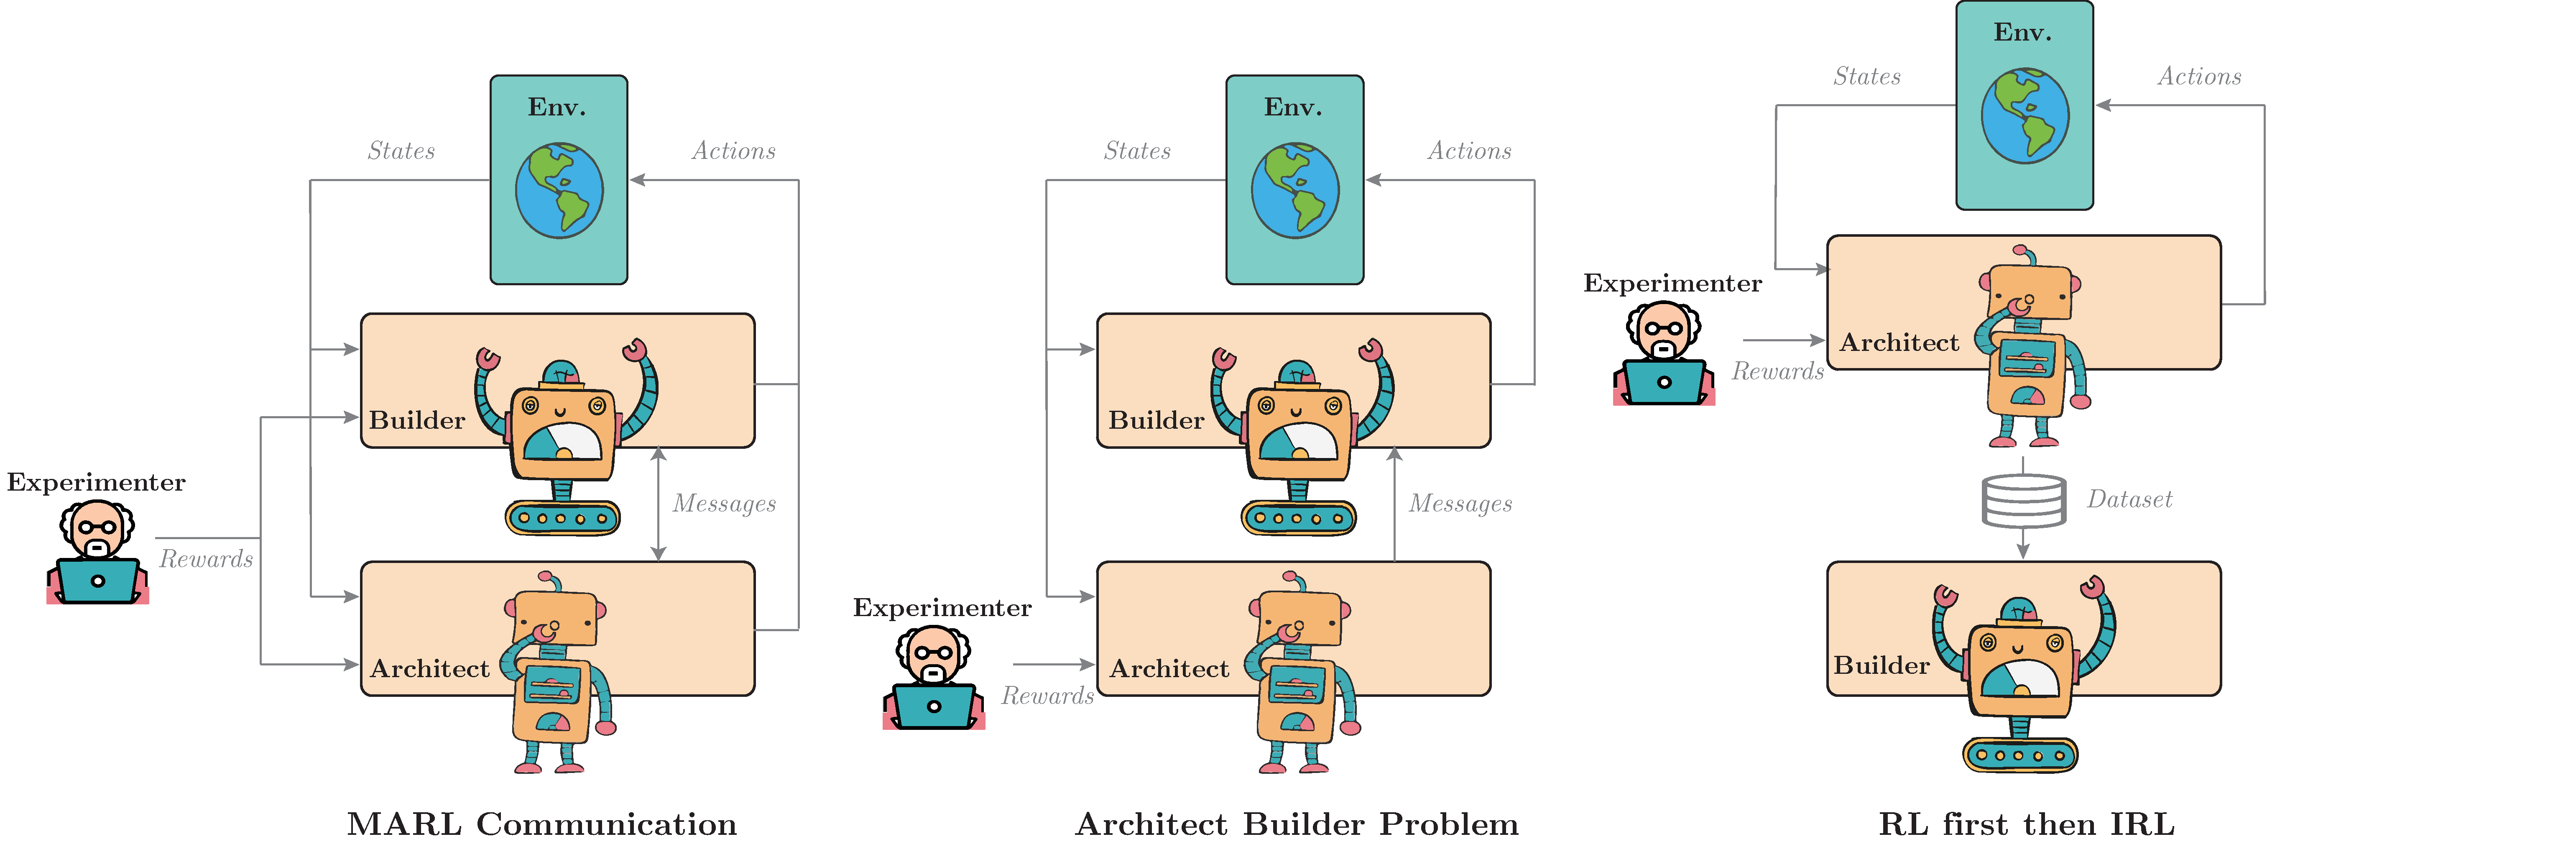
\includegraphics[width=\textwidth]{problem_def/prob_def_abp.pdf}
    \caption{The Architect Builder Problem and how it differs with respect to other \ai paradigms. Conversely to \marl communication (a), in \abp, the architect cannot act in the environment and the builder never perceives the reward (b). Because the architect cannot act in the environment, it is impossible to frame the problem as an \rl and then \irl problem (c).}
    \label{fig:prob_def_abp}
\end{figure}

The \abp is in fact a computational implementation of an experimental semiotics investigation: the Coconstruction Game~\citep{vollmer2014studying}. In their experiment, the builder and the architect are humans. They are located in separate rooms. The architecture has a picture of a target lego block structure while the builder is seated at a table in front of a set of lego blocks. The architect monitors the builder workspace via a camera (video stream) and must send messages to the builder until it manages to construct the structure. In order to prevent pre-existing communication systems from influencing the results of their studies, the architect uses a button box with neutral symbols (designed to minimize the presence of biases such as color or shape, so as to avoid the attribution of preexisting meanings).
We explore the \abp in chapter~\ref{chap:abig}. More specifically, we propose an algorithmic solution to it in a construction environment like the Coconstruction Game. We investigate the key learning dynamics in terms of mutual information between messages and actions and show that agents can agree on a communication protocol enabling them to generalize to new constructions never seen during training.


%---------------------------------------------------------------------------------------------------%
%---------------------------------------------------------------------------------------------------%
%---------------------------------------------------------------------------------------------------%
%---------------------------------------------------------------------------------------------------%
\newpage

\section{Self-organisation of Trajectories: the Open-ended Skill Acquisition Problem}
\label{sec:self-orga-traj}
%

\subsection{Computational Models of the Formation of Skill Repertoires with Autotelic RL}
\label{sec:self-orga-traj-context}
Beyond modeling Language formation, developmental \ai aims to model how children learn skills in general. In this study, we propose a computational framework that addresses the challenge of self-organizing developmental trajectories and the open-ended learning of skill repertoires. The framework, referred to as autotelic \rl or developmental \rl, is a combination of developmental approaches and reinforcement learning (see the definition of autotelic in \sect{sec:humans_autotelic}).  It builds on \textit{intrinsic motivations} (\ims) to enable agents to learn to represent, generate, select, and solve their own problems. To provide a comprehensive understanding of the framework, we first present a typology of intrinsic motivation approaches in developmental \ai, followed by a presentation of the autotelic learning problem and its solution with autotelic agents.
\paragraph{Intrinsic Motivations in Developmental AI}

 Developmental \ai aims to model children learning and, thus, takes inspiration from the mechanisms underlying autonomous behaviors in humans. Most of the time, humans are not motivated by external rewards but spontaneously explore their environment to discover and learn about what is around them. This behavior is driven by \textit{intrinsic motivations} (\ims) a set of brain processes that motivate humans to explore for the mere purpose of experiencing novelty, surprise or learning progress~\citep{berlyne1966curiosity,gopnik1999scientist,kidd2015psychology,oudeyer2016evolution,gottlieb2018towards}. 
 
 The integration of \ims into artificial agents thus seems to be a key step towards autonomous learning agents \citep{schmidhuber1991possibility,kaplan2007search}. In developmental robotics, this approach enabled sample efficient learning of high-dimensional motor skills in complex robotic systems \citep{santucci2020intrinsically}, including locomotion \citep{baranes2013active,martius2013information}, soft object manipulation \citep{rolf2013efficient,nguyen2014socially}, visual skills \citep{lonini2013robust} and nested tool use in real-world robots \citep{imgep}. Most of these seminal approaches leverage \textit{population-based} optimization algorithms, i.e. non-parametric models trained on (outcome, policy) pairs. These methods train separate policies for each goal, often demonstrate limited generalization capabilities, and cannot easily handle high-dimensional perceptual spaces.

Recently, we have been observing a convergence between developmental robotics and deep \rl, forming a new domain that we propose to call \textit{developmental reinforcement learning} as a subfield of developmental \ai. Indeed, \rl researchers now incorporate fundamental ideas from the developmental robotics literature in their own algorithms, and reversely developmental robotics learning architectures are beginning to benefit from the generalization capabilities of deep \rl techniques. These convergences can mostly be categorized in two ways depending on the type of intrinsic motivation (\ims) being used \citep{oudeyer2007intrinsic}:
\begin{itemize}
    \item
    \textbf{Knowledge-based IMs} are about prediction. They compare the situations experienced by the agent to its current knowledge and expectations and reward it for experiencing dissonance (or resonance). This family includes \ims rewarding prediction errors \citep{schmidhuber1991possibility,pathak2017curiosity}, novelty \citep{bellemare2016unifying,burda2018exploration,raileanu2020ride}, surprise \citep{achiam2017surprise}, negative surprise \citep{berseth2019smirl}, learning progress \citep{lopes2012exploration,kim2020active} or information gains \citep{houthooft2016vime}, see a review in \citep{linke2019adapting}. This type of \im is often used as an auxiliary reward to organize the exploration of agents in environments characterized by sparse rewards. It can also be used to facilitate the construction of world models \citep{lopes2012exploration,kim2020active,sekar2020planning}.
    \item
    \textbf{Competence-based IMs}, on the other hand, are about control. They reward agents to solve self-generated problems, to achieve self-generated goals. In this category, agents need to represent, select and master self-generated goals. As a result, competence-based \ims were often used to organize the acquisition of repertoires of skills in task-agnostic environments \citep{baranes2010intrinsically,baranes2013active,santucci2016grail,forestier2016modular,nair2018visual,warde2018unsupervised,curious,blaes2019control,pong2019skew}.
    % Just like knowledge-based \ims, competence-based \ims organize the exploration of the world and, thus, might be used to train world models \citep{baranes2013active,chitnis2020glib} or facilitate learning in sparse reward settings \citep{geppg}. We propose to use the adjective \textbf{autotelic}, from the Greek \textit{auto} (self) and \textit{telos} (end, goal), to characterize agents that are intrinsically motivated to represent, generate, pursue and master their own goals (\ie that are both intrinsically motivated and goal-conditioned).
\end{itemize}

\begin{figure}[!h]
\centering
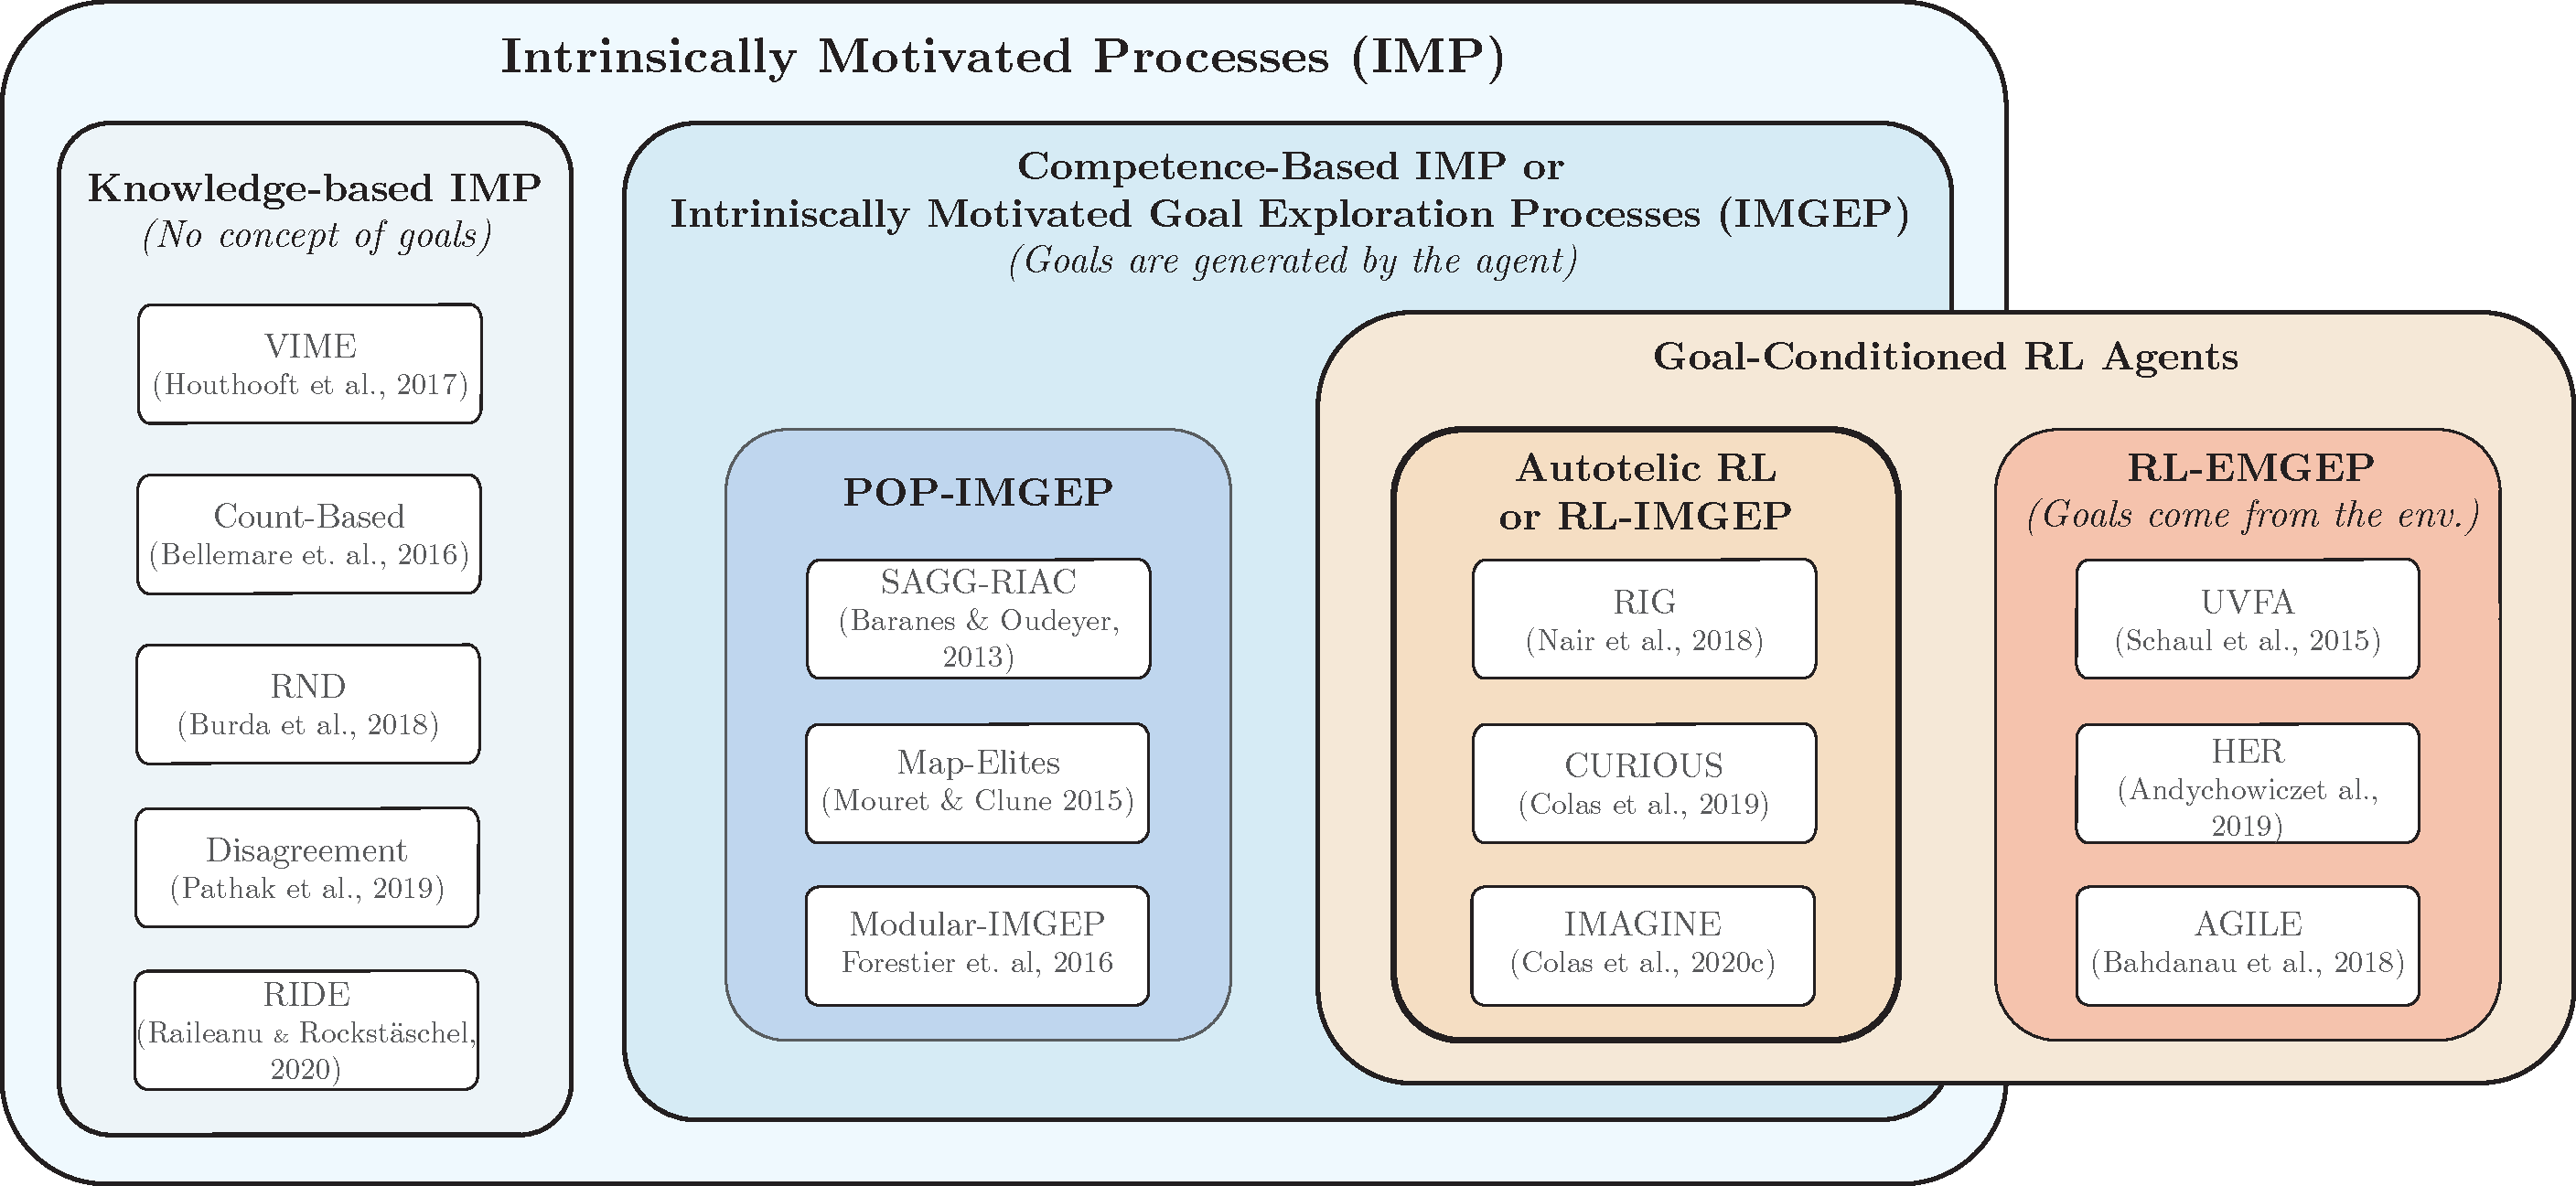
\includegraphics[width=.95\textwidth]{survey/scope_survey.pdf}
\caption{A typology of intrinsically-motivated and/or goal-conditioned \rl approaches. \popimgep, \rlimgep and \rlemgep refer to population-based intrinsically motivated goal exploration processes, \rl-based \imgep and \rl-based externally motivated goal exploration processes respectively.}
\label{fig:survey_scope}
\end{figure}


Figure~\ref{fig:survey_scope} proposes a visual representation of intrinsic motivations approaches (knowledge-based \ims vs competence-based \ims or \imgeps) and \rl approaches (intrinsically vs externally motivated). \rl algorithms using \textit{knowledge-based} \ims (on the left) leverage ideas from developmental robotics to solve standard \rl problems. On the other hand, algorithms using competence-based \ims organize exploration around self-generated goals and can be seen as targeting a developmental robotics problem: the \textit{open-ended formation of skill repertoires}. \textit{Intrinsically Motivated Goal Exploration Processes} (\imgep) is the family of autotelic algorithms that bake competence-based \ims into learning agents \citep{imgep}. \imgep agents generate and pursue their own goals as a way to explore their environment, discover possible interactions, and build repertoires of skills. This framework emerged from the field of developmental robotics \citep{oudeyer2007intrinsic,baranes2009proximo,baranes2010intrinsically,rolf2010goal} and originally leveraged population-based learning algorithms (\popimgep) \citep{baranes2009r,baranes2013active,forestier2016modular,imgep}. The intersection between \imgep and multi-goal \rl are autotelic \rl algorithms or \rlimgep. They train agents to generate and pursue their own goals by training goal-conditioned policies. They contrast with \rlemgep agents which do not generate their own goals and rely on externally provided ones. 



\paragraph{The Autotelic Learning problem}

In the \textit{autotelic learning problem} or the \textit{open-ended formation of skill repertoires}, the agent is set in an open-ended environment without any pre-defined goal and needs to acquire a repertoire of skills. Here, we use the definition of skill provided in \sect{sec:background_mg_rl}, i.e. the association of a goal embedding $z_g$ and the policy to reach it $\Pi_g$. A repertoire of skills is thus defined as the association of a repertoire of goals $\m{G}$ with a goal-conditioned policy trained to reach them $\Pi_\m{G}$. The intrinsically motivated skills acquisition problem can now be modeled by a reward-free \mdp $\m{M}\,=\,\{\m{S},\, \m{A},\, \m{T},\, \rho_0\}$ that only characterizes the agent, its environment and their possible interactions. Just like children, agents must be autotelic, \ie they should learn to represent, generate, pursue, and master their own goals. \Fig{fig:rl_vs_autotelic} illustrates the key difference between multi-goal \rl (\sect{sec:background_mg_rl}) and autotelic \rl. In multi-goal \rl an experimenter provides goals and rewards to the agent. 
%
\begin{figure}[!h]
\centering
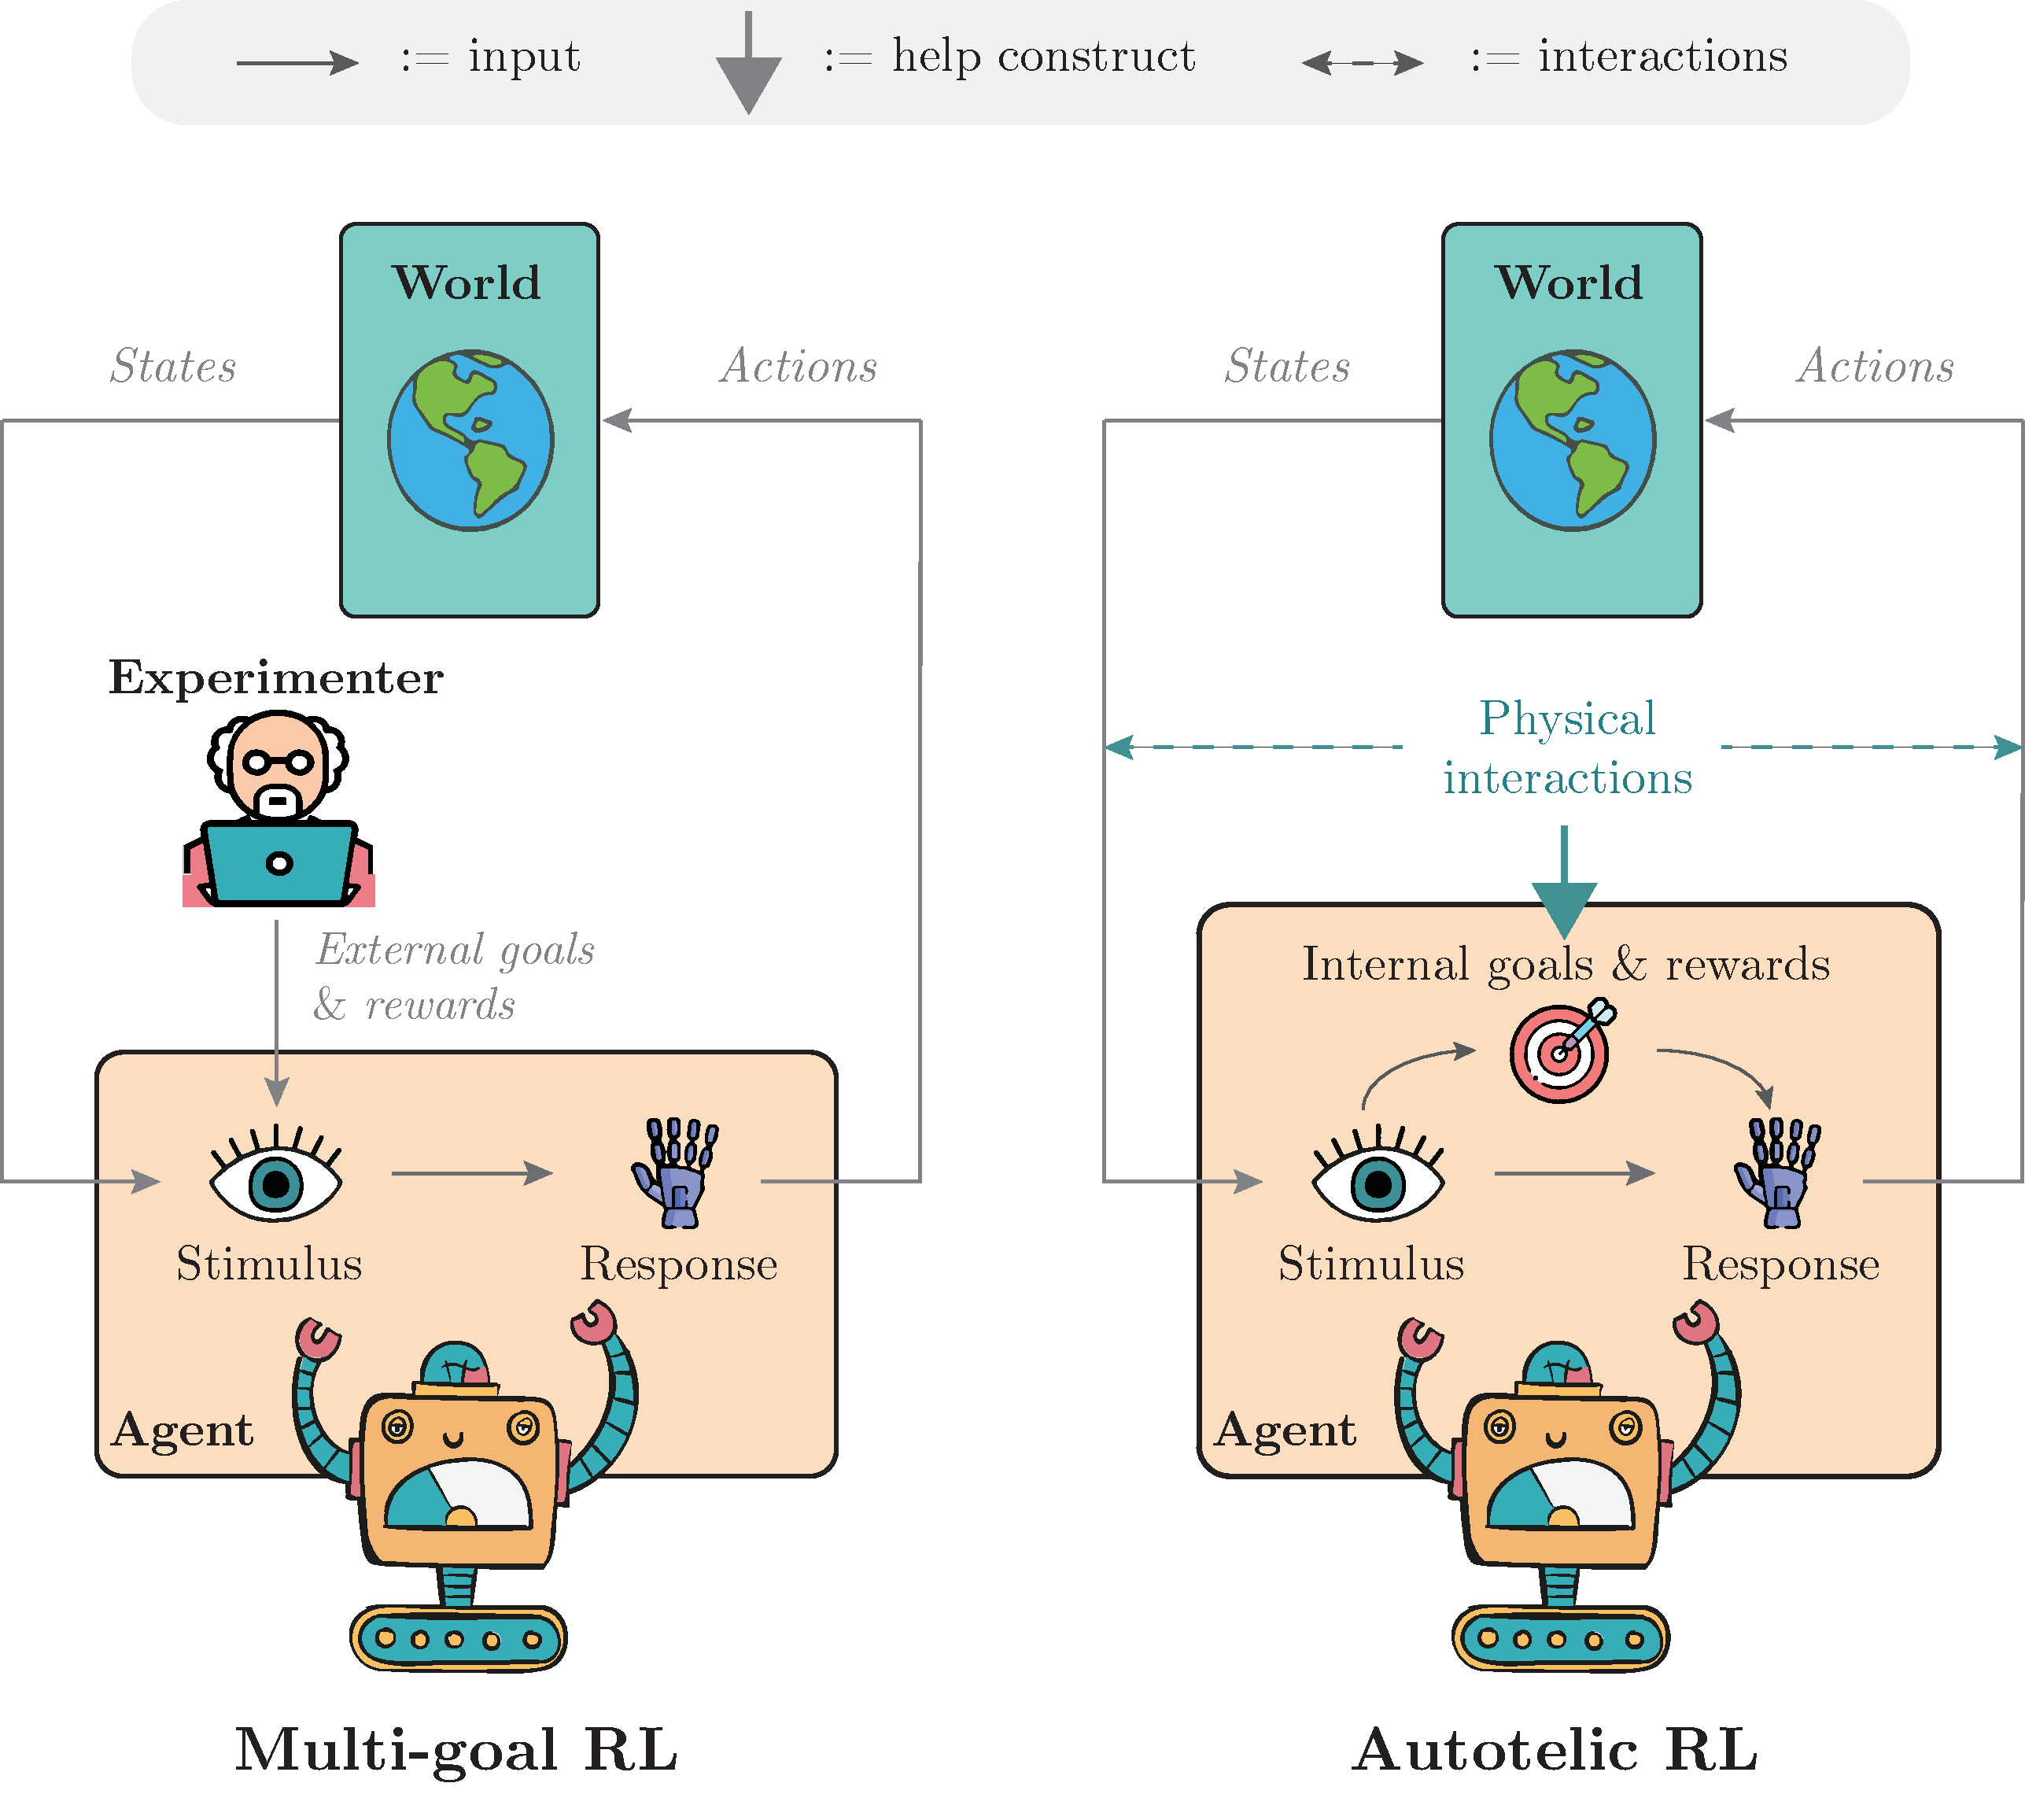
\includegraphics[width=.62\textwidth]{problem_def/autotelic_rl_interactions.pdf}
\caption{Multi-goal \rl vs Autotelic \rl: In autotelic \rl, agents learn to represent, generate, pursue and master their own goals. Goals are thus internal to the agent while multi-goal \rl relies on an external experimenter providing goals and rewards.}
\label{fig:rl_vs_autotelic}
\end{figure}

\paragraph{Evaluating Autotelic Agents}

Evaluating agents is often trivial in reinforcement learning. Agents are trained to maximize one or several pre-coded reward functions\,---\,the set of possible interactions is known in advance. One can measure generalization abilities by computing the agent's success rate on a held-out set of testing goals. One can measure exploration abilities via several metrics such as the count of task-specific state visitations.

In contrast, autotelic agents evolve in open-ended environments and learn to represent and form their own set of skills. In this context, the space of possible behaviors might quickly become intractable for the experimenter, which is perhaps the most interesting feature of such agents. For these reasons, designing evaluation protocols is not trivial. The evaluation of such systems raises similar difficulties as the evaluation of task-agnostic content generation systems like Generative Adversarial Networks (\gan) \citep{goodfellow2014generative} or self-supervised language models \citep{devlin2019bert,brown2020language}. In both cases, learning is \textit{task-agnostic} and it is often hard to compare models in terms of their outputs (\eg comparing the quality of \gan output images, or comparing output repertoires of skills in autotelic agents).

\begin{itemize}[noitemsep]
    \item \textbf{Measuring exploration:} one can compute task-agnostic exploration proxies such as the entropy of the
    visited state distribution, or measures of state coverage (\eg coverage of the high-level x-y state space in mazes) \citep{goalgan}. Exploration can also be measured as the number of interactions from a set of \textit{interesting} interactions defined subjectively by the experimenter (interactions with objects as we do in chapter~\ref{chap:imagine}).
    \item \textbf{Measuring generalization:} The experimenter can define a set of relevant target goals
    and prevent the agent from training on them. Evaluating agents on this held-out set at test time provides a measure of generalization \citep{ruis2020benchmark}, although it is biased towards what the experimenter assesses as \textit{relevant} goals.
    \item \textbf{Measuring transfer learning:} The intrinsically motivated exploration of the environment can be seen as a pre-training phase to bootstrap learning in a subsequent downstream task. In the downstream task, the agent is trained to achieve externally-defined goals. We report its performance and learning speed on these goals. This is akin to the evaluation of self-supervised language models, where the reported metrics evaluate performance in various downstream tasks \citep{brown2020language}. 
    \item \textbf{Opening the black-box:} Investigating internal representations learned during intrinsically motivated exploration is often informative. One can investigate properties of the goal generation system (\eg does it generate out-of-distribution goals?), investigate properties of the goal embeddings (\eg are they disentangled?). One can also look at the learning trajectories of the agents across learning, especially when they implement their own curriculum learning \citep{goalgan,curious,blaes2019control,pong2019skew,akakzia2020decstr}.
    \item \textbf{Measuring robustness:} Autonomous learning agents evolving in open-ended environment should be robust to a variety of properties than can be found in the real-world. This includes very large environments, where possible interactions might vary in terms of difficulty (trivial interactions, impossible interactions, interactions whose result is stochastic thus prevent any learning progress). Environments can also include distractors (\eg non-controllable objects) and various forms of non-stationarity. Evaluating learning algorithms in various environments presenting each of these properties allows to assess their ability to solve the corresponding challenges.
\end{itemize}

\paragraph{Autotelic RL Agents}

\rlimgep are intrinsically motivated versions of goal-conditioned \rl algorithms. They need to be equipped with mechanisms to represent and generate their own goals in order to solve the autotelic learning problem. Concretely, this means that, in addition to the goal-conditioned policy, they need to learn: 1)~to represent goals $g$ by compact embeddings $z_g$; 2)~to represent the support of the goal distribution, also called \textit{goal space} $\m{Z}_\m{G}=\{z_g\}_{g\in\m{G}}$; 3)~a goal distribution from which targeted goals are sampled $\m{D}(z_g)$; 4)~a goal-conditioned reward function $\m{R}_\m{G}$. This four modules are illustrated in \fig{fig:inside_autotelic_agents}. In practice, only a few architectures tackle the four learning problems above. Indeed, simple autotelic agents assume pre-defined goal representations (1), the support of the goals distribution (2) and goal-conditioned reward functions (4). As autotelic architectures tackle more of the 4 learning problems, they become more and more advanced. As we will see in the following sections, many existing works in goal-conditioned \rl can be formalized as autotelic agents by including goal sampling mechanisms \textit{within the definition of the agent}. 
\begin{figure}[!h]
\centering
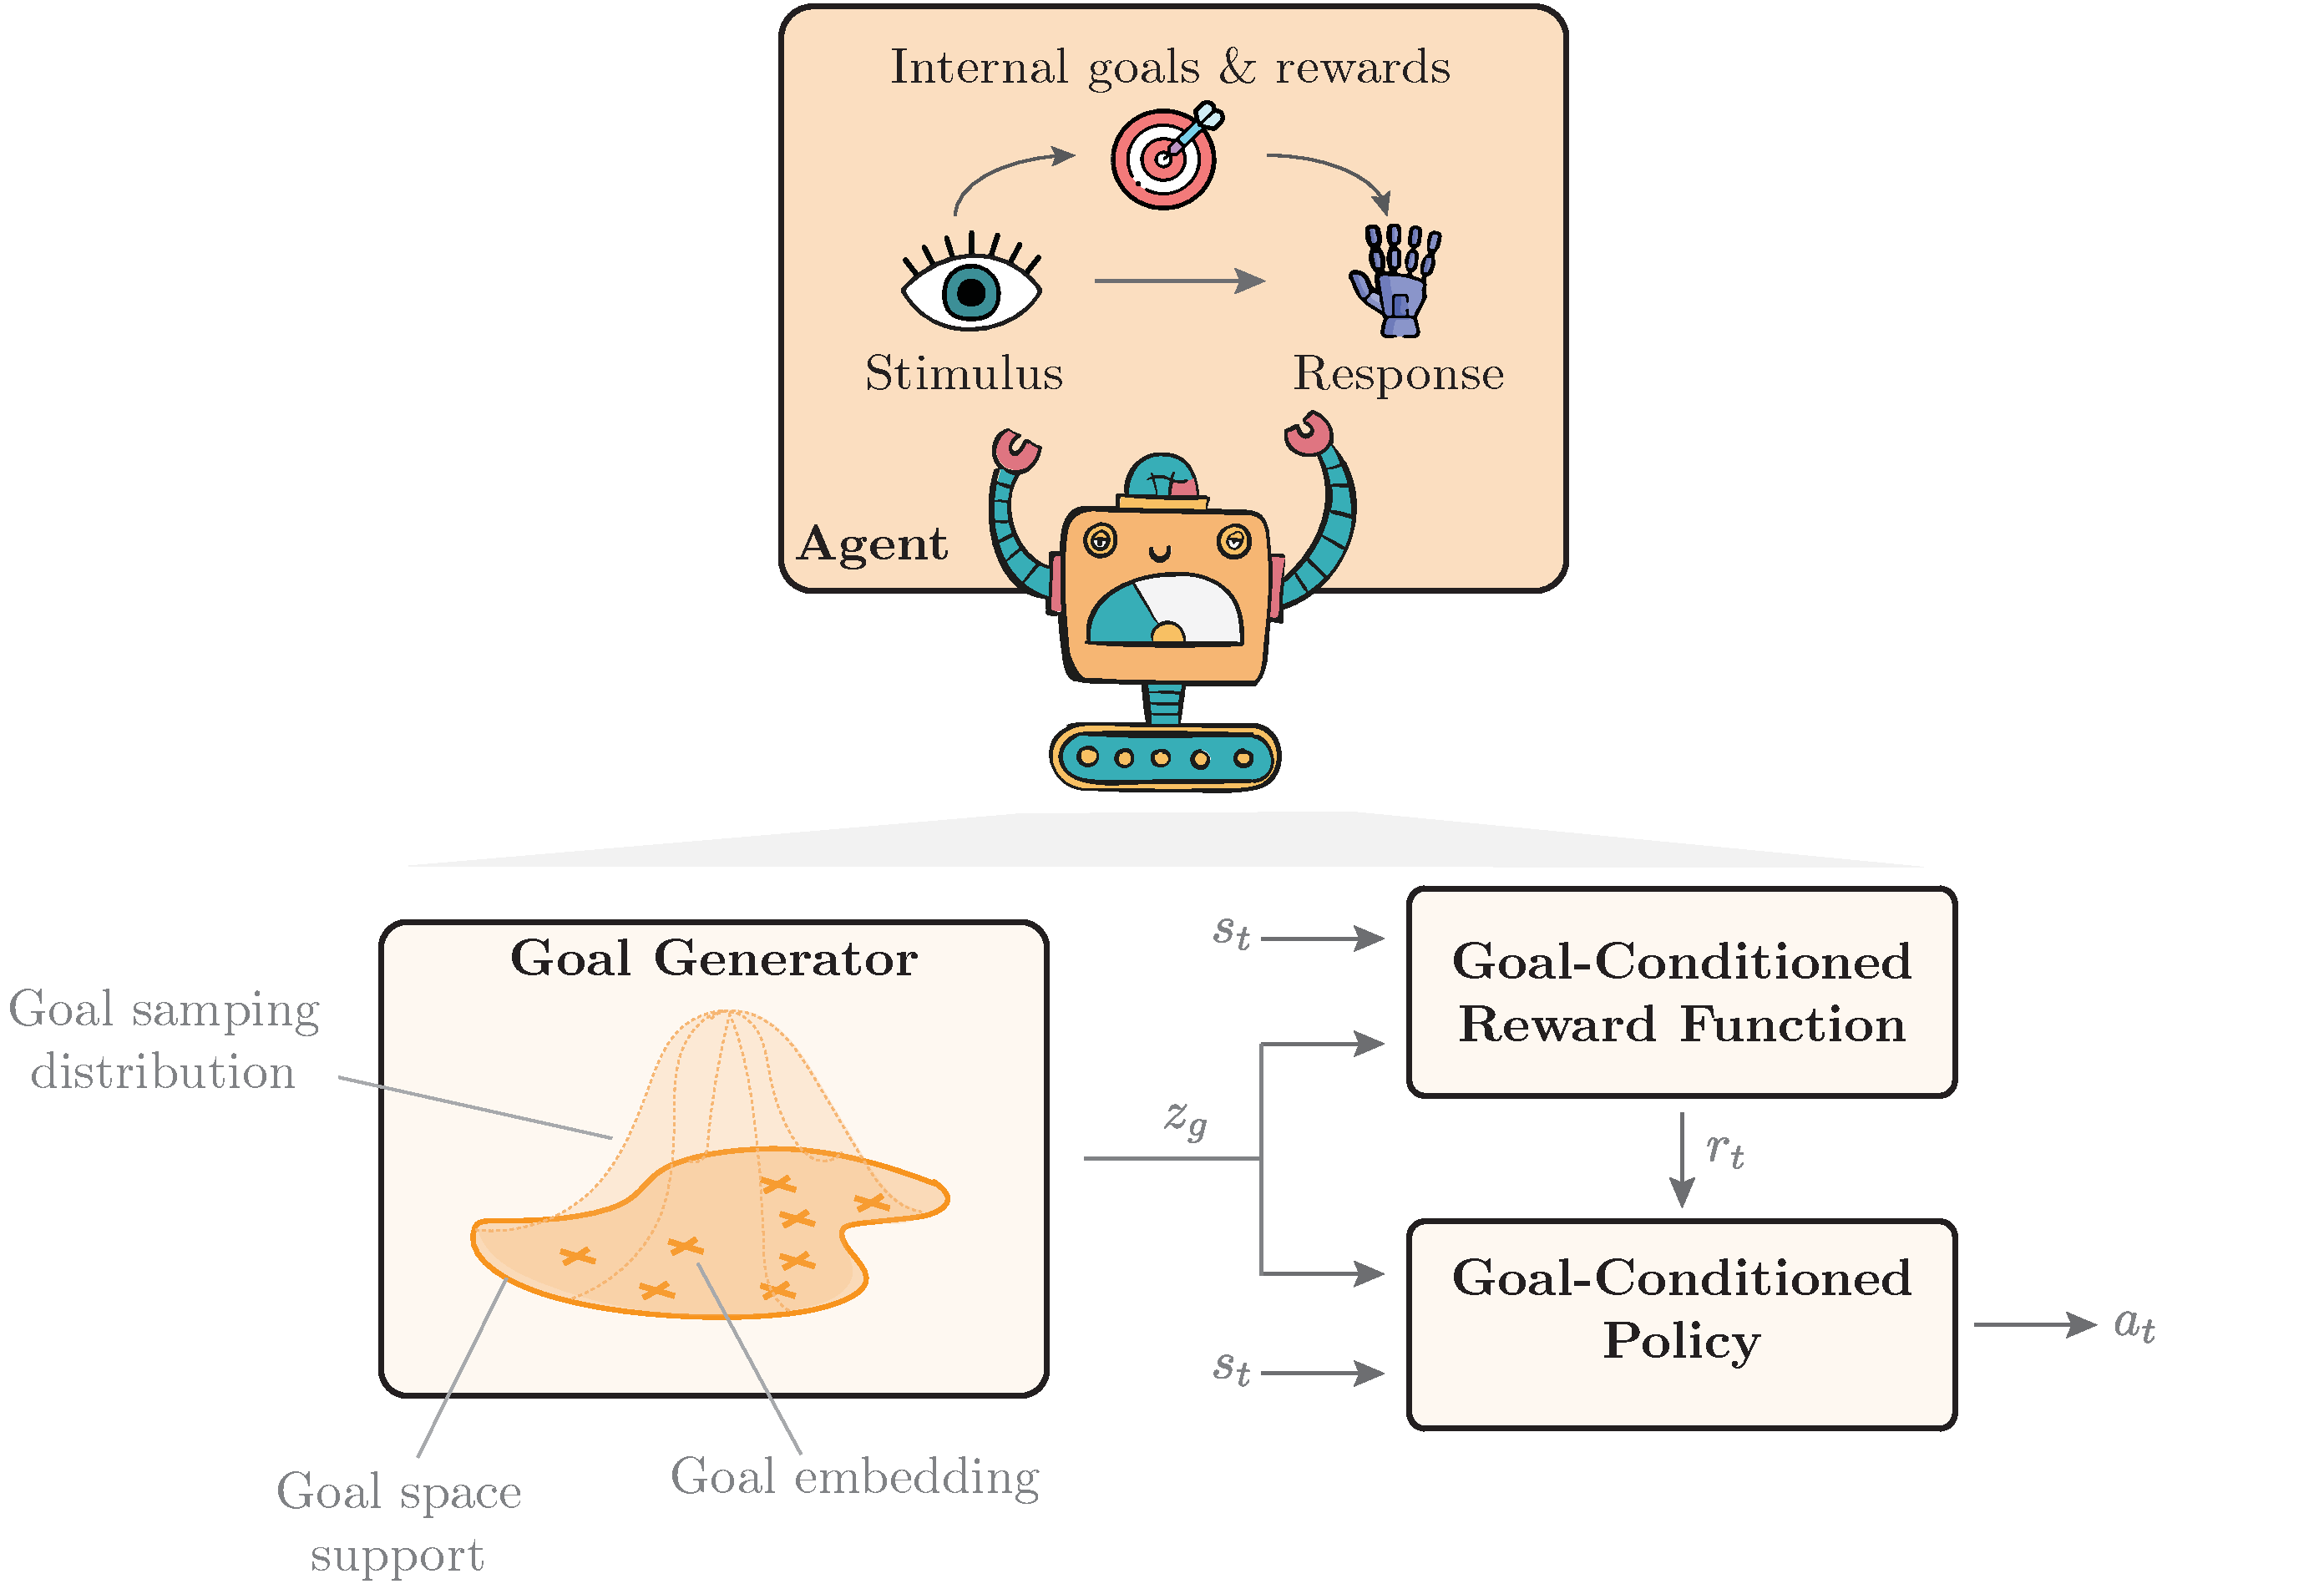
\includegraphics[width=.75\textwidth]{problem_def/inside_autotelic_agent.pdf}
\caption{Representation of the different learning modules in an autotelic agent. }
\label{fig:inside_autotelic_agents}
\end{figure}

Algorithm~\ref{algo:IMGEP} details the pseudo-code of \rlimgep algorithms. Starting from randomly initialized modules and memory, \rlimgep agents enter a standard \rl interaction loop. They first observe the context (initial state), then sample a goal from their goal sampling policy. Then starts the proper interaction. Conditioned on their current goal embedding, they act in the world so as to reach their goal, \ie to maximize the cumulative rewards generated by the goal-conditioned reward function. After the interaction, the agent can update all its internal models. It learns to represent goals by updating its goal embedding function and goal-conditioned reward function, and improves its behavior towards them by updating its goal-conditioned policy. 

\noindent\begin{minipage}{\textwidth}
   \centering
   \begin{minipage}{.6\textwidth}
        \begin{algorithm}[H]
            \small
        	\caption{~ Autotelic Agent with RL-IMGEP}
        	\label{algo:IMGEP}
        	\begin{algorithmic}[1]
            	\REQUIRE environment $\m{E}$
            	\STATE \textbf{Initialize} empty memory $\m{M}$,goal-conditioned policy $\Pi_\m{G}$, goal-conditioned reward $R_\m{G}$,goal space $\m{Z}_\m{G}$, goal sampling policy $GS$.
            	
            	\LOOP
            	
%                \LineCommentConttwo{\textit{Observe context}}
                \STATE Get initial state: $s_0 \leftarrow \m{E}$.reset()
%            	\LineCommentCont{\textit{Sample goal}}
            	\STATE Sample goal embedding $z_g=GS(s_0, \m{Z}_\m{G})$.
%            	\LineCommentCont{\textit{Roll-out goal-conditioned policy}}
            	\STATE Execute a roll-out with $\Pi_g=\Pi_\m{G}(\cdot \mid z_g)$
            	\STATE Store collected transitions $\tau=(s,a,s')$ in $\m{M}$.
%            	\LineCommentCont{\textit{Update internal models}}
                \STATE Sample a batch of $B$ transitions: $\m{M}\sim \{(s,a,s')\}_B$.
                \STATE Perform Hindsight Relabelling $\{(s,a,s',z_g)\}_B$.
                \STATE Compute internal rewards $r=R_\m{G}(s,a,s'\mid z_g)$.
            	\STATE Update policy $\Pi_\m{G}$ via \rl on $\{(s,a,s',z_g,r)\}_B$.
            	\STATE Update goal representations  $\m{Z}_\m{G}$. 
            	\STATE Update goal-conditioned reward function $R_\m{G}$. 
            	\STATE Update goal sampling policy $GS$.
            	\ENDLOOP
            	\STATE \Return $\Pi_\m{G}, R_\m{G}, \m{Z}_\m{G}$
        	\end{algorithmic}
        \end{algorithm}
   \end{minipage}
   \hspace{0.2cm}
   \begin{minipage}{.37\textwidth}
  \textbf{ } \\
  \\
        \centering
        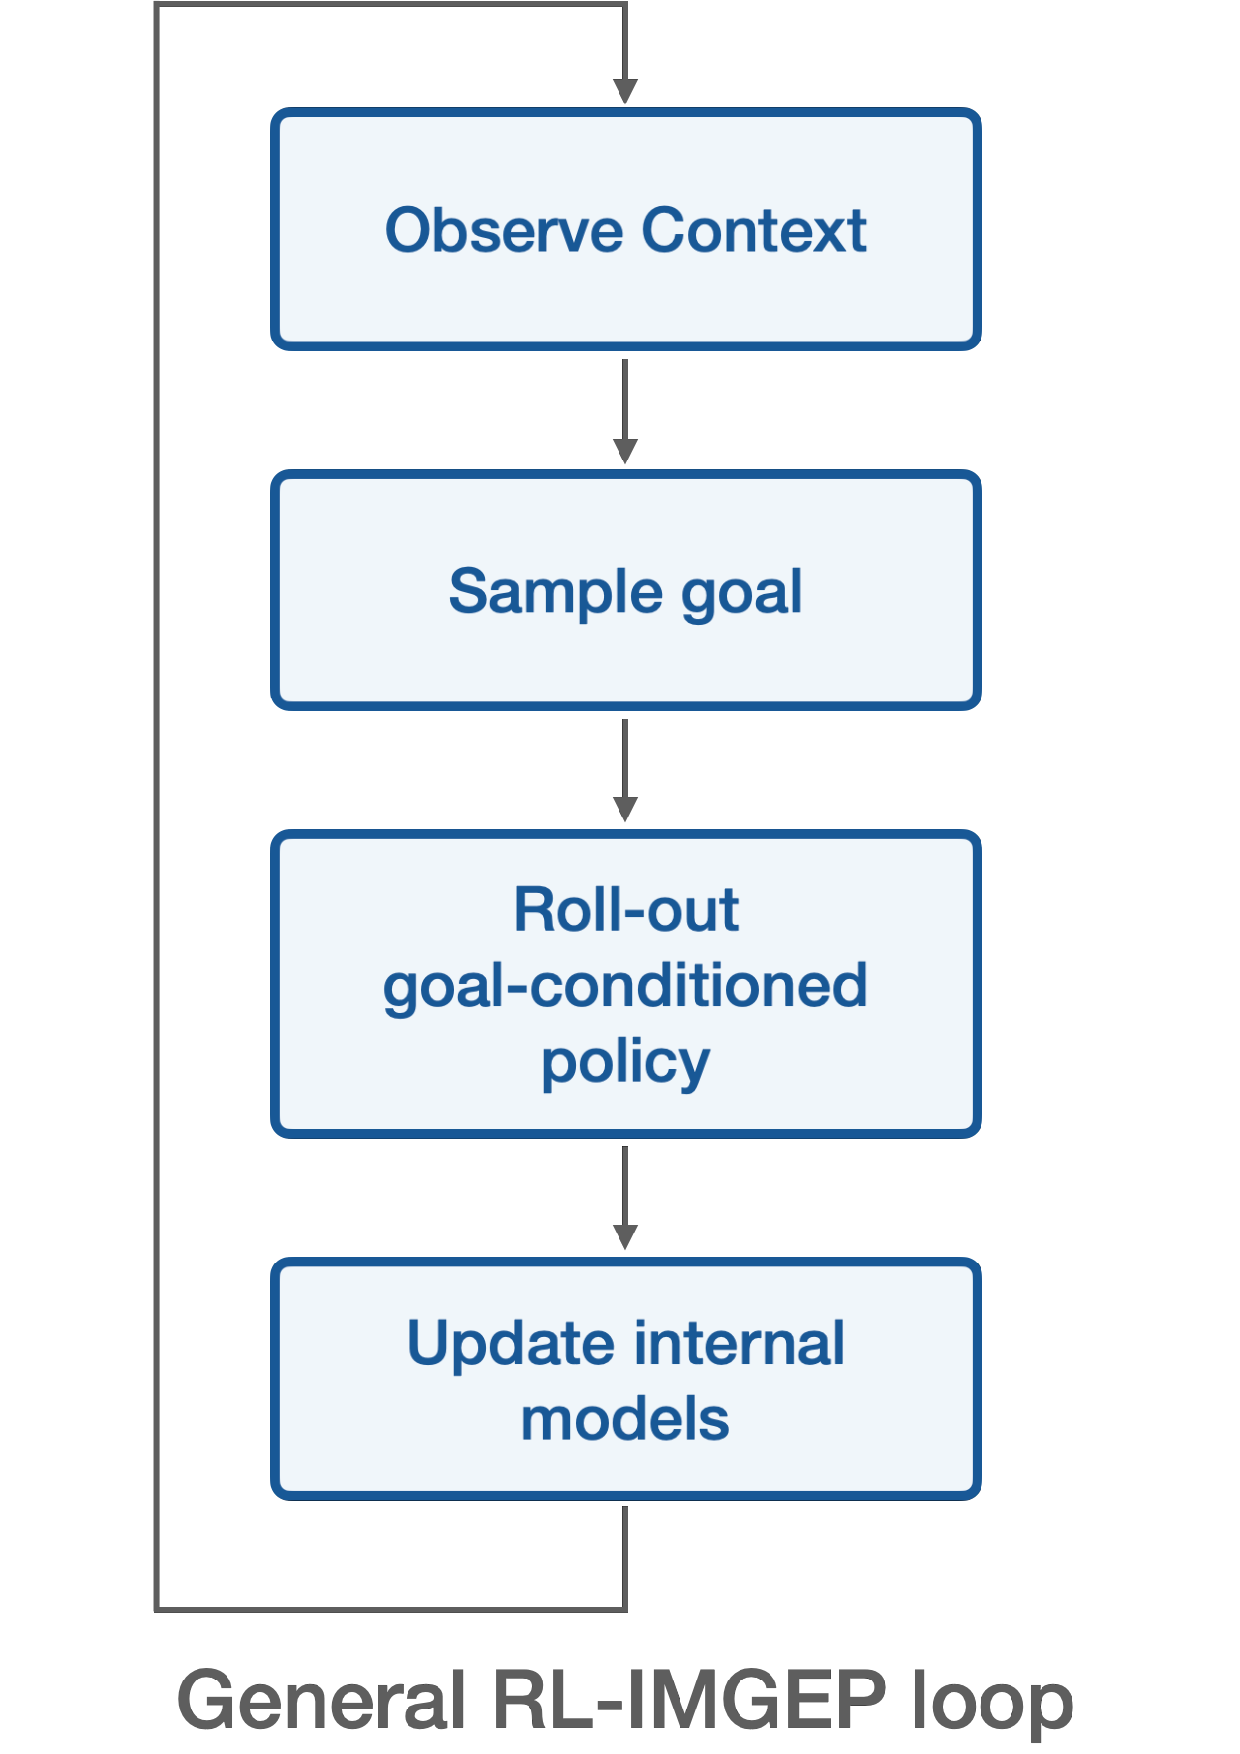
\includegraphics[width=0.9\textwidth]{survey/loop-algo.pdf}
    \end{minipage}
   \label{fig:test}
\end{minipage}
    


Most \rlemgep approaches use pre-defined goal representations where goal spaces and associated rewards are pre-defined by the engineer and are part of the task definition (see our topology of goal representation in \sect{sec:background_mg_rl}). On the other hand, autotelic agents actually need to learn these goal representations. While individual goals are represented by their embeddings and associated reward functions, representing multiple goals also requires the representation of the \textit{support} of the goal space, \ie how to represent the collection of \textit{valid goals} that the agent can sample from, see \fig{fig:inside_autotelic_agents}. In addition to constructing a goal space, autotelic agents must sample goals within that space to actually explore the world. The next two sections address the questions of how to learn goal representations and how to select goals. 

\paragraph{How to Learn Goal Representations?}

\noindent\textbf{Learning Goal Embeddings.} Some approaches assume the pre-existence of a goal-conditioned reward function, but learn to represent goals by learning goal embeddings. This is the case of language-based approaches, which receive rewards from the environment (thus are \rlemgep), but learn goal embeddings jointly with the policy during policy learning \citep{Hermann2017,chan2019actrce,Jiang2019,bahdanau2018systematic,hill2019emergent,ther,lynch2020grounding}. When goals are target images, goal embeddings can be learned via generative models of states, assuming the reward to be a fixed distance metric computed in the embedding space \citep{nair2018visual,florensa2019selfsupervised,pong2019skew,nair2020contextual}.

\noindent\textbf{Learning reward functions.} A few approaches go even further and learn their own goal-conditioned reward function. In the domain of image-based goals, \citet{venkattaramanujam2019self,hartikainen2019dynamical} learn a distance metric estimating the square root of the number of steps required to move from any state $s_1$ to any $s_2$ and generates internal signals to reward agents for getting closer to their target goals. \citet{warde2018unsupervised} learn a similarity metric in the space of controllable aspects of the environment that is based on a mutual information objective between the state and the goal state $s_g$. This method is reminiscent of \textit{empowerment} methods \cite{mohamed_variational_2015,gregor2016variational,achiam_variational_2018,eysenbach2018diversity,dai_empowerment-based_2020,sharma_dynamics-aware_2020,choi_variational_2021}. Empowerment methods aim at maximizing the mutual information between the agent's actions or goals and its experienced states. Recent methods train agents to develop a set of skills leading to maximally different areas of the state space. Agents are rewarded for experiencing states that are easy to discriminate, while a discriminator is trained to better infer the skill $z_g$ from the visited states. This discriminator acts as a skill-specific reward function. 

In the domain of language goals, \citet{bahdanau2018learning,imagine} learn language-conditioned reward functions from an expert dataset or from language descriptions of autonomous exploratory trajectories respectively. However, the \textsc{agile} approach from \citet{bahdanau2018learning} does not generate its own goals.  

 \noindent\textbf{Learning the supports of goal distributions.} Finally, to represent collections of goals, agents need to represent the support of the goal distribution\,---\,which embeddings correspond to valid goals and which do not. To this end, most approaches consider a pre-defined, bounded goal space in which any point is a valid goal (\eg target positions within the boundaries of a maze, target block positions within the gripper's reach)~\citep{schaul2015universal,andrychowicz2017hindsight,nair2017overcoming,plappert2018multi,curious,blaes2019control,lanier2019curiosity,ding_imitation_2019,li2019towards}. However, not all approaches assume pre-defined goal spaces. However, some approaches use the set of previously experienced representations to form the support of the goal distribution \citep{veeriah2018many,akakzia2020decstr,ecoffet2020first}. In \citet{goalgan}, a Generative Adversarial Network (\gan) is trained on past representations of states ($\varphi(s)$) to model a distribution of goals and thus its support. In the same vein, approaches handling image-based goals usually train a generative model of image states based on Variational Auto-Encoders (\vae) to model goal distributions and support \citep{nair2018visual,pong2019skew,nair2020contextual}. In both cases, valid goals are the one generated by the generative model.

\paragraph{How to Select Goals?}

Once autotelic agents have constructed a goal support inside a goal space, they need to specify a goal selection policy. Although agents can sample their goal space uniformly, informed goal selection can be a way for agents to organize their learning curriculum automatically.

\noindent\textbf{Automatic curriculum learning (\acl).} Applied for goal selection, \acl is a mechanism that organizes goal sampling so as to maximize long-term performance improvement (distal objective). As this objective is usually not directly differentiable, curriculum learning techniques usually rely on a proximal objective. Proxies include \textit{intermediate difficulty}~\citep{sukhbaatar2017intrinsic,campero2020learning,zhang2020automatic}, \textit{novelty-diversity}~\citep{warde2018unsupervised,pong2019skew,pitis2020maximum,kovac2020grimgep,Fang-RSS-21} or \textit{medium-term learning progress}~\citep{baranes2013active,moulinfriergmm,forestier2016modular,fournier2018accuracy,fournier2019clic,curious,blaes2019control,portelas_teacher_2020}. Interested readers can refer to \citet{portelas2020automatic}, which present a broader review of \textsc{acl} methods.

\noindent\textbf{Hierarchical reinforcement learning (\hrl).} \hrl can be used to guide the sequencing of goals \citep{dayan1993feudal,sutton1998intra,sutton_between_1999,precup2001temporal}. In \hrl, a high-level policy is trained via \rl or planning to generate sequence of goals for a lower level policy so as to maximize a higher-level reward. This allows to decompose tasks with long-term dependencies into simpler sub-tasks. Low-level policies are implemented by traditional goal-conditioned \rl algorithms \citep{levy2018hierarchical,roder2020curious} and can be trained independently from the high-level policy \citep{kulkarni2016hierarchical,frans2017meta} or jointly \citep{levy2018hierarchical,nachum2018data,roder2020curious}.

\paragraph{Summary}
In this section, we presented the autotelic \rl framework. This paradigm, at the intersection of developmental robotics and standard \ai technics, builds intrinsically motivated agents that generate and pursue their own problems. Autotelic agents fall in the category of competence-based \ims. Unlike standard multi-goal \rl agents that rely on externally provided goals, autotelic agents discover and learn to represent their own goals from their experience of the physical world. This ability to develop in symbiosis with the physical world is reminiscent of Piaget's developmental psychology~\citep{piaget1952origins} which highlights children's ability to shape their learning trajectories with respect to their sensory-motor experience of the world. 
 
\subsection{Problem Definition}
\label{sec:problem-def-vygo}

In the second part of this manuscript, we will investigate the role of cultural conventions in the self-organization of agents' developmental trajectories. To do so, we will extend the autotelic \rl framework presented in the previous section (\sect{sec:self-orga-traj-context}). Complementing the Piagetian approach of autotelic \rl and inspired by the literature deriving from \citet{vygotsky_thought_1934}'s theory of child development, we propose a new framework called \textit{Vygotskian Autotelic \ai}.

The initial contribution of Part~\ref{part:exploitation} is conceptual. It proposes to draw the contours of an \ai framework where agents leverage pre-existing cultural conventions to transform their learning abilities. It is important to note that, in contrast with the first portion of this research, this investigation will examine the scenario of artificial agents using pre-established cultural conventions to organize their developmental trajectories, disregarding any negotiation of protocols or multi-agent dynamics. In Vygotksian Autotelic agents do not only interact with the physical world surrounding them but with social partners. They are immersed in a (rich) sociocultural environment. An illustration of the difference between autotelic \rl and Vygotskian autotelic \rl is provided in \fig{fig:towards_vygo_rl}. In \sect{sec:vygo_aai}, 

\begin{figure}[!h]
    \centering
    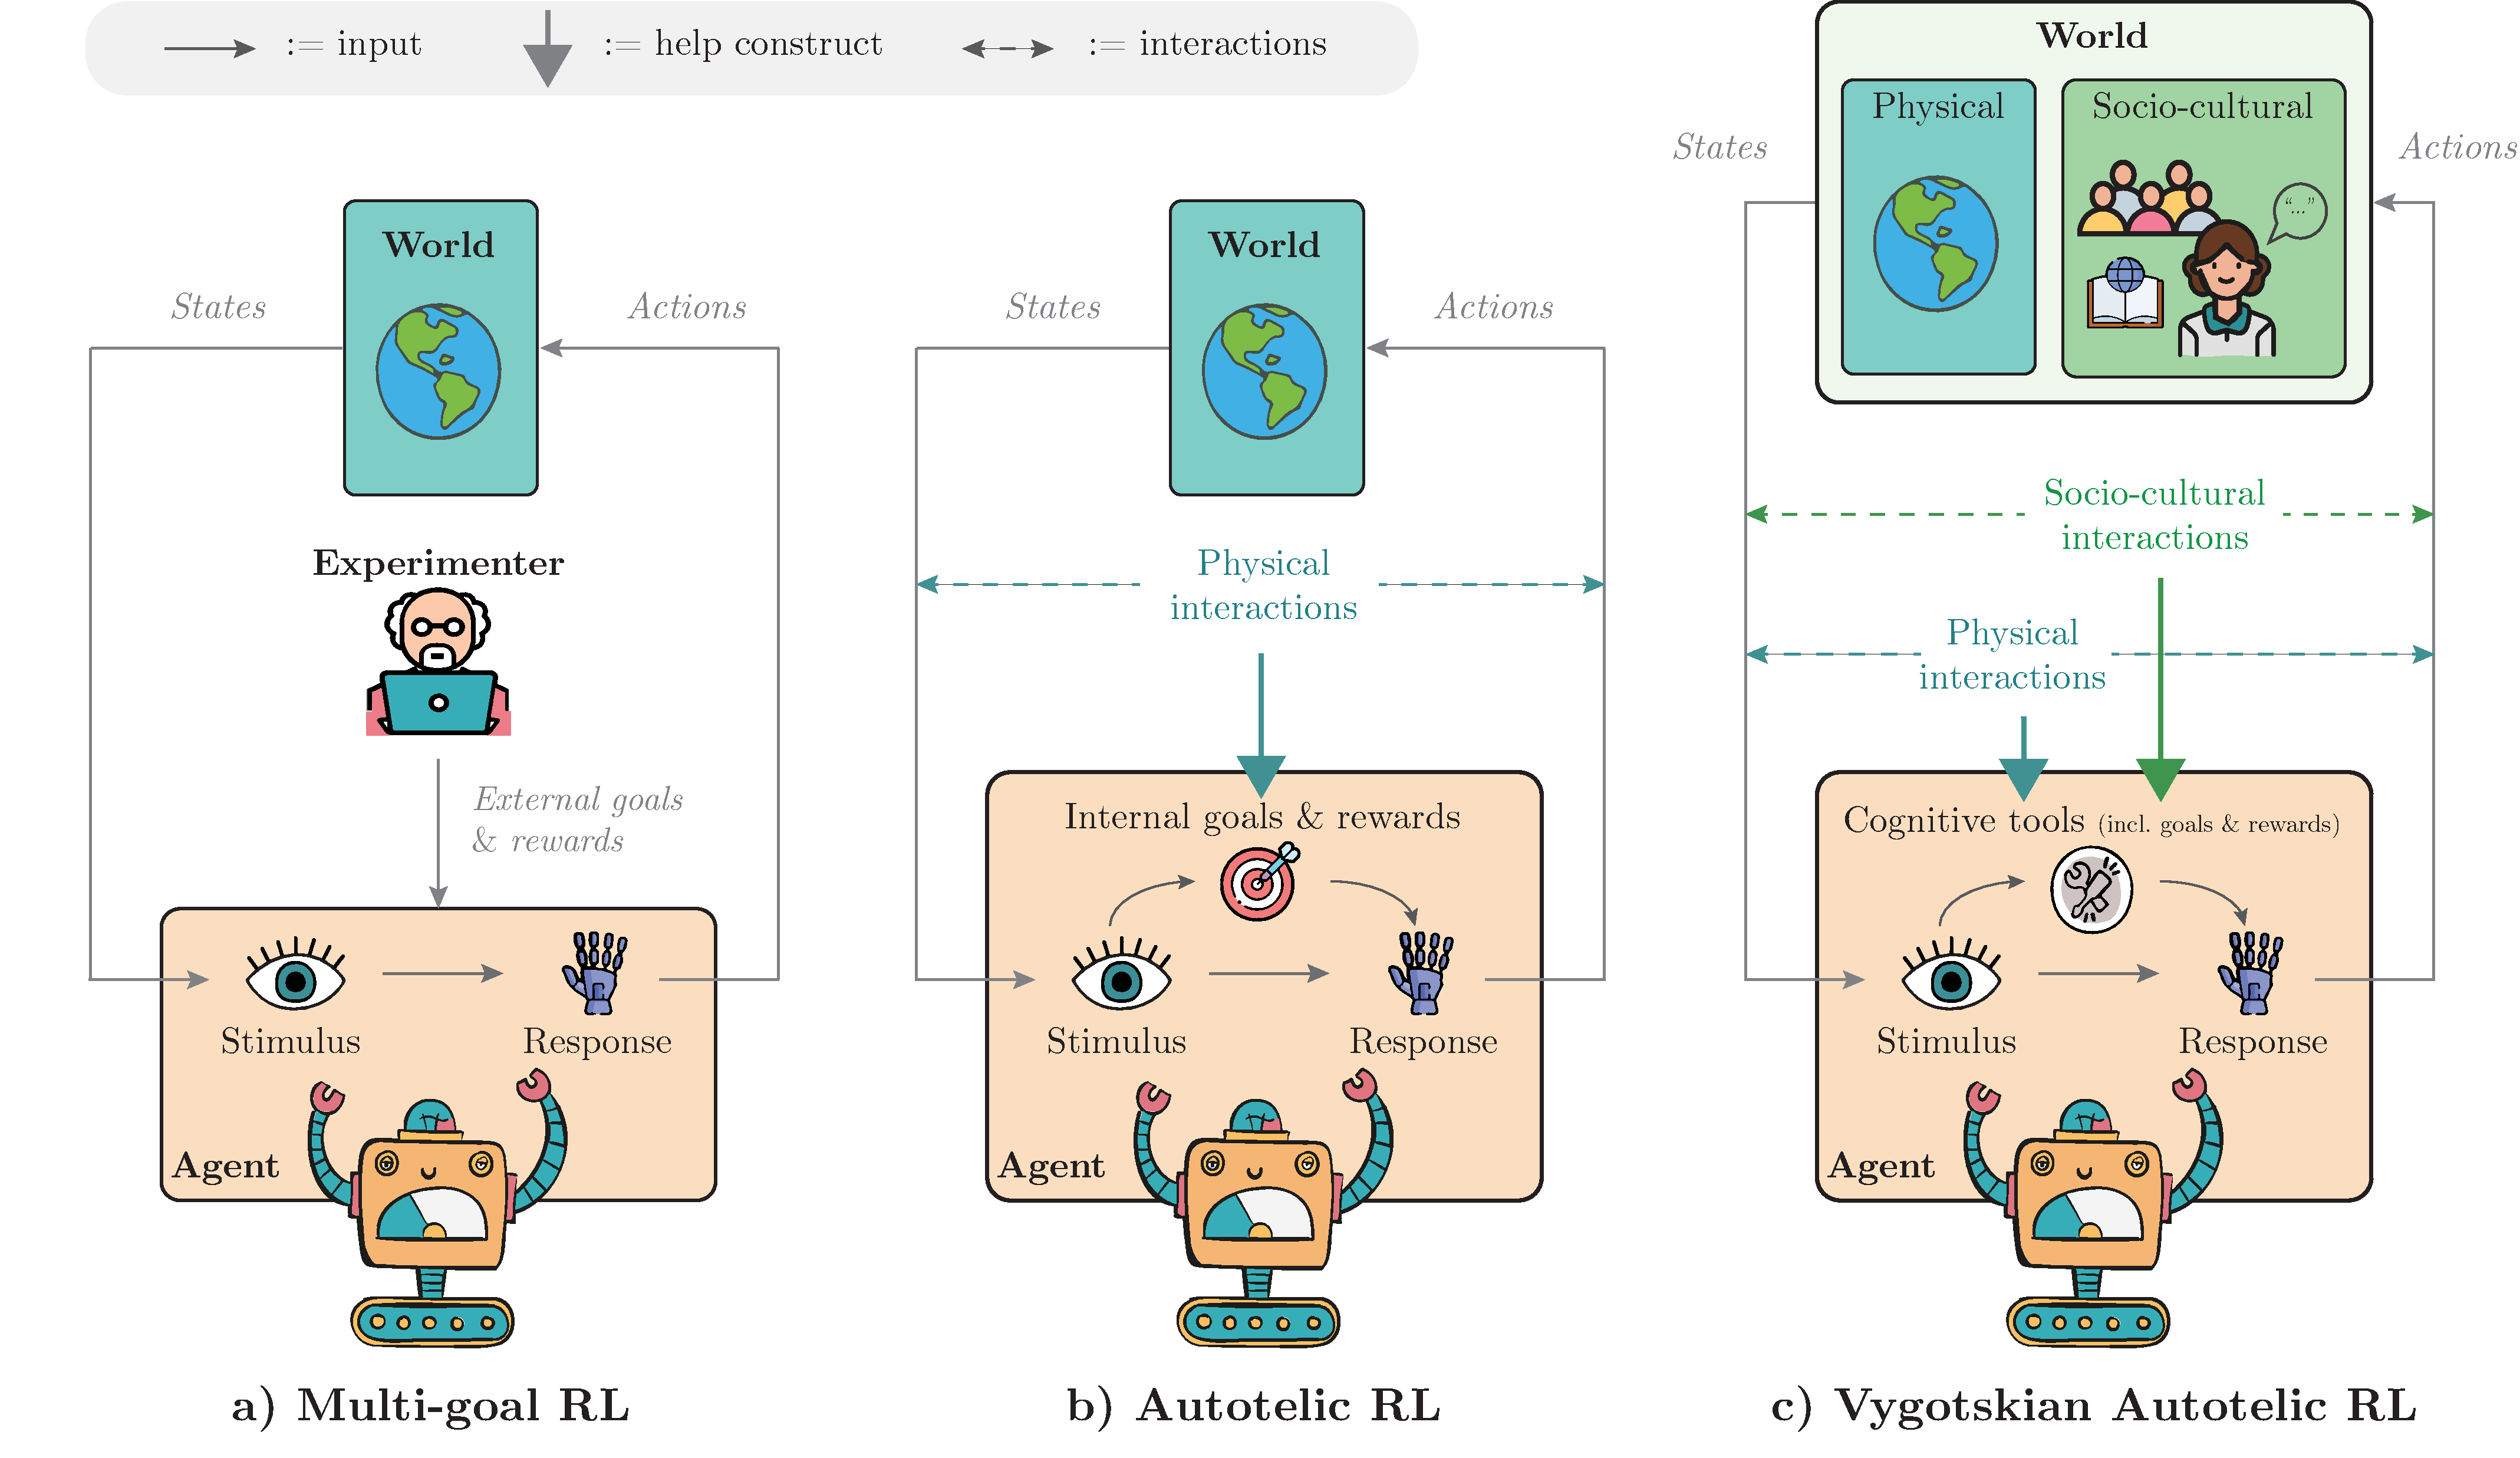
\includegraphics[width=\textwidth]{figures/perspective/figure-intro-v4.pdf}
    \caption{From multi-goal RL to autotelic RL to Vygotskian autotelic RL. \rl defines an agent experiencing the state of the world as stimuli and acting on that world via actions. Multi-goal RL (a): goals and associated rewards come from pre-engineered functions and are perceived as sensory stimuli by the agent. Autotelic RL (b): agents build internal goal representations from interactions between their intrinsic motivations and their physical experience (Piagetian view). Vygotskian autotelic RL (c): agents internalise physical and socio-cultural interactions into \textit{cognitive tools}. Here, \textit{cognitive tools} refer to any self-generated representation that mediates stimulus and actions: self-generated goals, explanations, descriptions, attentional biases, visual aids, mnemonic tricks, etc. }
    \label{fig:towards_vygo_rl}
\end{figure}

To benefit from sociocultural and linguistic conventions, Vygotksian autotelic agents need to ground them into their own sensory-motor modalities. They need to extract the structure of language and align it with their sensory-motor experience. As will be discussed, agents do not merely extract the structure of language, but instead assimilate the entire convention, generating an internal representation of the social partner with whom they are interacting. This internal model can be called at any time to generate plans in an autotelic fashion for instance. We argue that this Vygotskian framework can palliate autotelic agents' serious limitations in terms of goal diversity, exploration, generalization, or skill composition. To back this claim, we present two experimental contributions displaying how agents can ground complex spatiotemporal language (\sect{sec:grounding}) and how they can use language as a cognitive tool to generate goals in curiosity-driven exploration (\sect{sec:imagine}). Both of these experimental contributions will leverage the \textit{Playground} environment: a socio-physical environment made of a variety of objects with different properties and a simulated social partner providing linguistic descriptions of interesting interactions. \todo{give more details on experimental contribs}




